\chapter{Autonomous Driving as a Representative Application}
\label{sec:application}
% ============================================


% Springer Nature: each chapter should have a 10--15 line online abstract.
% This chapter abstract has not yet been written in the uploaded manuscript.
\abstract{Autonomous driving is used in this chapter as a representative, end-to-end instance of the sensor-fusion principles developed in Chapters~\ref{sec:classicalSF} and~\ref{sec:learning}. We first describe the sensor suite of a modern vehicle, with indicative orders of magnitude for update rate, range, accuracy and dominant error sources of cameras, LiDAR, radar, ultrasonic sensors, inertial units, wheel odometry and GNSS, and we discuss field-of-view coverage and redundancy. We then formalise the alignment steps that every fusion pipeline relies on: extrinsic calibration as a rigid transform in $SE(3)$, projection of LiDAR points into images, timestamp interpolation, ego-motion compensation of rotating LiDAR sweeps and the handling of delayed or out-of-sequence measurements, including a quantitative account of how calibration and synchronisation errors propagate into fused estimates. Two runnable worked examples with real numbers anchor the core fusion tasks: ego-localisation by GNSS--IMU--wheel-odometry fusion through a tunnel outage, and object-level camera--radar track fusion with naive independent fusion and covariance intersection. The chapter closes with the public datasets and evaluation metrics of the field (AP, NDS, IoU, MOTA/AMOTA, ATE/RPE, NEES/NIS and ECE), the latency, middleware and determinism aspects of deployment, and end-of-chapter problems with solutions and companion code.}
\suppressfloats[t]

Autonomous driving is a representative high-complexity application of sensor fusion because it brings together heterogeneous sensing, real-time operation, uncertainty management, safety-critical decision-making, and strict deployment constraints. It is not the only domain in which sensor fusion is required, but it provides a particularly useful case study because many general fusion challenges appear simultaneously within a complete cyber--physical system. In this chapter, autonomous driving is therefore used to illustrate how the theoretical principles and algorithmic methods discussed in the previous sections are instantiated in practice. The chapter is organised as follows: the sensor suite and its indicative characteristics; the alignment steps (calibration, synchronisation, ego-motion compensation) that precede any fusion; the core fusion tasks, two of which are developed as runnable worked examples that reuse the estimators of Chapter~\ref{sec:classicalSF}; the datasets and metrics by which fusion systems are evaluated; and the implementation and validation aspects that connect the algorithms to a deployed vehicle, with pointers to the learning-based methods of Chapter~\ref{sec:learning}, the multi-agent fusion of Chapter~\ref{sec:MAS} and the open challenges of Chapter~\ref{sec:open-challenges}.

\section{System Context and Sensor Suite}

An autonomous vehicle must estimate both its external environment and its own state. To do so, it combines exteroceptive sensors, which observe the surrounding scene; proprioceptive sensors, which measure ego-motion; and external or cooperative information sources, which provide global, map-based, or communication-assisted context. A representative sensor arrangement is shown in Fig.~\ref{fig:autonomous-vehicle-sensors-layout}.

\begin{figure}[!t]
    \centering
    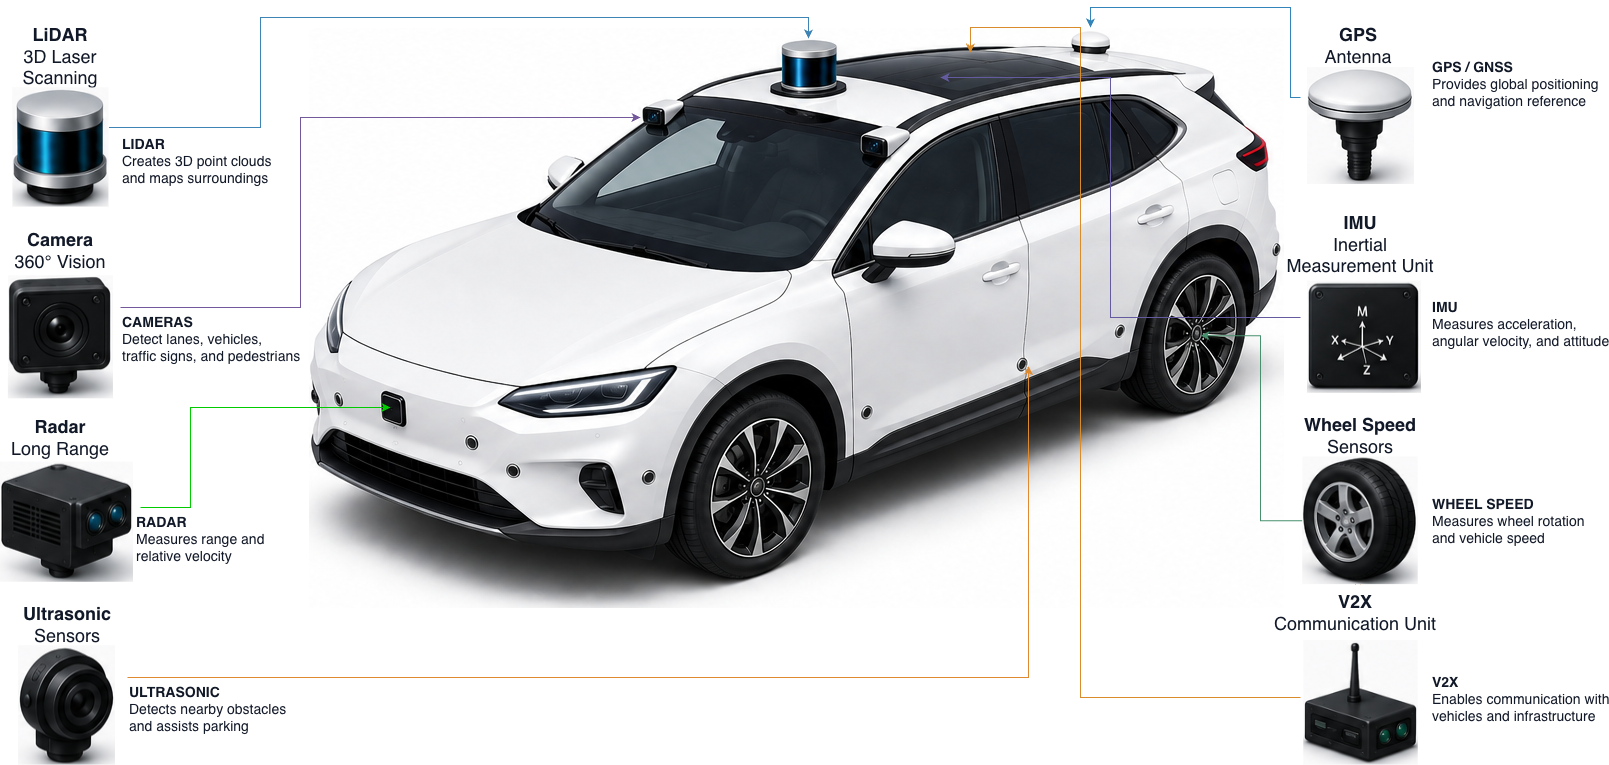
\includegraphics[width=\textwidth]{figures/autonomous_vehicle_sensors_layout_v02.png}
    \caption{Representative autonomous-vehicle sensor layout, showing complementary sensing modalities for perception, localisation, ego-motion estimation, short-range obstacle detection, and communication.}
    \label{fig:autonomous-vehicle-sensors-layout}
\end{figure}

The sensor layout in Fig.~\ref{fig:autonomous-vehicle-sensors-layout} highlights the complementarity that motivates autonomous-driving sensor fusion. The strengths, limitations, and typical fusion roles of the individual modalities are summarised in Tables~\ref{tab:av-onboard-sensors} and~\ref{tab:av-cooperative-inputs}; here we only note the overall pattern: cameras contribute semantics, LiDAR contributes geometry, radar contributes range and velocity under poor visibility, ultrasonic sensors cover the near field, IMUs and wheel odometry provide high-rate ego-motion subject to drift, and GNSS, maps, V2X, and roadside infrastructure extend awareness beyond the onboard field of view.

These modalities are not interchangeable. Instead, each provides a different type of information, with different uncertainty, sampling rate, field of view, latency, and failure modes. Autonomous-driving fusion therefore aims to exploit both \emph{complementarity}, where one sensor provides information that another cannot, and \emph{redundancy}, where multiple sensors observe related aspects of the same scene and can be used for consistency checking, robustness, and fault tolerance.

Table~\ref{tab:av-onboard-sensors} summarises common onboard sensing modalities, while Table~\ref{tab:av-cooperative-inputs} summarises cooperative, localisation, and map-based inputs that support autonomous-driving fusion.

\begin{table}[!t]
    \centering
    \small
    \caption{Onboard sensing modalities commonly used in autonomous-driving sensor fusion.}
    \label{tab:av-onboard-sensors}
    \begin{tabular}{p{0.08\linewidth} p{0.28\linewidth} p{0.30\linewidth} p{0.25\linewidth}}
        \hline
        \textbf{Sensor} & \textbf{Strengths} & \textbf{Limitations} & \textbf{Typical Fusion Role} \\
        \hline
        Camera & Dense appearance, colour, texture, lane markings, traffic signs, traffic lights, and semantic cues & Sensitive to lighting, glare, shadows, night-time conditions, adverse weather, and limited direct depth estimation & Semantic perception, object classification, lane detection, traffic-light recognition, image--LiDAR and image--radar fusion \\
        \hline
        LiDAR & Accurate 3D geometry, depth, object shape, road structure, and point-cloud representation & Higher cost, sparse at long range, affected by rain, fog, snow, and reflective surfaces & 3D object detection, mapping, localisation, free-space estimation, camera--LiDAR fusion \\
        \hline
        Radar & Long range, direct relative velocity, robustness to poor visibility and adverse weather & Lower angular resolution, multipath effects, ghost detections, noisier spatial structure & Object tracking, velocity estimation, long-range detection, radar--camera and radar--LiDAR fusion \\
        \hline
        Ultrasonic & Low-cost short-range sensing, useful for parking and close obstacle detection & Very limited range, low spatial resolution, affected by surface geometry and environmental noise & Low-speed manoeuvring, parking assistance, near-field obstacle detection \\
        \hline
        IMU & High-rate acceleration and angular velocity, useful for short-term ego-motion estimation & Biases and integration drift accumulate over time & Ego-motion prediction, inertial navigation, GNSS--IMU, visual--inertial, and LiDAR--inertial fusion \\
        \hline
        Wheel odometry & Direct vehicle motion information, low cost, high update rate & Accumulates drift, affected by wheel slip, tyre deformation, and road surface conditions & Dead reckoning, vehicle state estimation, GNSS--IMU--odometry fusion \\
        \hline
    \end{tabular}
\end{table}

\begin{table}[!t]
    \centering
    \small
    \caption{Cooperative sensing, localisation, and map-based inputs used in autonomous-driving fusion.}
    \label{tab:av-cooperative-inputs}
    \begin{tabular}{p{0.13\linewidth} p{0.26\linewidth} p{0.28\linewidth} p{0.24\linewidth}}
        \hline
        \textbf{Input} & \textbf{Strengths} & \textbf{Limitations} & \textbf{Typical Fusion Role} \\
        \hline
        GNSS & Provides global positioning in open-sky environments and supports absolute localisation & Degraded by tunnels, urban canyons, multipath, signal blockage, interference, and spoofing risks & Global localisation, correction of accumulated drift in GNSS--IMU, GNSS--wheel odometry, and map-based localisation \\
        \hline
        High-definition maps & Provide prior information about lanes, road boundaries, intersections, landmarks, traffic rules, and road topology & Can become outdated, require accurate localisation, and are costly to build, update, and maintain & Map matching, lane-level localisation, perception priors, planning context, road-structure reasoning \\
        \hline
        V2X communication & Extends perception beyond line of sight and can provide information from nearby vehicles, infrastructure, and traffic-management systems & Depends on connectivity, latency, standardisation, trust, cyber-security, and communication coverage & Cooperative perception, hazard warning, traffic-signal information, occlusion handling, extended situational awareness \\
        \hline
        Roadside infrastructure sensors & Provide external viewpoints from fixed cameras, LiDARs, radars, or smart-city infrastructure & Require deployment and maintenance, depend on communication links, and raise calibration, synchronisation, privacy, and security issues & Infrastructure-assisted perception, validation, cooperative tracking, scenario recording, ground-truth-like reference generation \\
        \hline
    \end{tabular}
\end{table}

\subsection{Indicative Sensor Characteristics}
\label{subsec:sensor-characteristics}

Tables~\ref{tab:av-onboard-sensors} and~\ref{tab:av-cooperative-inputs} are qualitative. Fusion design, however, needs numbers: the choice of filter rates, gating thresholds, process- and measurement-noise covariances and fallback strategies all depend on how fast, how far and how accurately each sensor observes the world. Table~\ref{tab:av-sensor-characteristics} therefore collects \emph{indicative orders of magnitude} for the sensors of Fig.~\ref{fig:autonomous-vehicle-sensors-layout}. The figures are representative of automotive-grade devices of the early 2020s and vary considerably with product, configuration and operating conditions \cite{yeong2021_sensors,patole2017_radar,groves2013_gnss}; they should be read as the starting point of a sensor-model identification, not as specifications.

\begin{table}[!t]
    \centering
    \scriptsize
    \caption{Indicative characteristics of automotive sensors (orders of magnitude; actual values depend on the product, the configuration and the operating conditions). $1\sigma$ accuracies refer to a single measurement in nominal conditions.}
    \label{tab:av-sensor-characteristics}
    \begin{tabular}{>{\raggedright\arraybackslash}p{0.15\linewidth} >{\raggedright\arraybackslash}p{0.10\linewidth} >{\raggedright\arraybackslash}p{0.13\linewidth} >{\raggedright\arraybackslash}p{0.24\linewidth} >{\raggedright\arraybackslash}p{0.28\linewidth}}
        \hline
        \textbf{Sensor} & \textbf{Update rate} & \textbf{Range} & \textbf{Resolution / accuracy} & \textbf{Main error sources} \\
        \hline
        Camera (mono, stereo, surround fisheye) & 10--60\,Hz & semantic: $>$200\,m; depth: 20--100\,m (stereo), poorer for mono & 1--8\,Mpx; angular resolution 0.02--0.1$^{\circ}$/pixel; mono range error 10--20\,\% of range & Illumination, glare, night, rain and fog, lens soiling, rolling shutter, calibration drift, depth ambiguity \\
        \hline
        Spinning or solid-state LiDAR & 10--20\,Hz & 100--250\,m (10\,\% reflectivity) & range $\pm$2--3\,cm; angular 0.1--0.4$^{\circ}$; 32--128 layers & Rain, fog and snow backscatter, blooming on retro-reflectors, motion distortion within a sweep, sparse returns at long range, dark or specular surfaces \\
        \hline
        77-GHz radar (long-range, corner, imaging) & 10--20\,Hz & 150--250\,m (long-range); 50--100\,m (corner) & range 0.1--0.5\,m; range rate $\pm$0.1\,m/s; azimuth 1--5$^{\circ}$ (0.1--1$^{\circ}$ imaging); poor elevation \added{except for 4D imaging radar} & Multipath and ghost targets, clutter, angular ambiguity, low resolution of extended objects, interference between radars \\
        \hline
        Ultrasonic & 10--40\,Hz & 0.2--5\,m & $\pm$1--3\,cm range, very coarse bearing & Temperature and wind, surface geometry and absorption, cross-talk, limited range \\
        \hline
        IMU, automotive MEMS grade & 100--1000\,Hz & -- & gyro bias instability 1--10$^{\circ}$/h, angle random walk 0.1--0.5$^{\circ}/\sqrt{\mathrm{h}}$; accelerometer bias 1--10\,mg & Bias (turn-on and in-run), scale factor, axis misalignment, temperature sensitivity, vibration; errors integrate into drift \\
        \hline
        IMU, tactical / navigation grade & 100--1000\,Hz & -- & bias instability 0.1--1$^{\circ}$/h (tactical), $<$0.01$^{\circ}$/h (navigation) & As above with smaller magnitude; cost, size and export restrictions limit automotive use \\
        \hline
        Wheel odometry & 50--100\,Hz & -- & speed $\pm$0.05--0.2\,m/s; scale error 1--2\,\% (tyre radius, pressure, load) & Slip and skid, surface, tyre deformation, quantisation at low speed, no direct heading \\
        \hline
        GNSS, single frequency & 1--10\,Hz & global & 2--5\,m horizontal (open sky) & Multipath, atmospheric delay, blockage in tunnels and urban canyons, interference and spoofing \\
        \hline
        GNSS, RTK / PPP-RTK & 1--20\,Hz & global & 1--3\,cm $+$ 1\,ppm (fixed solution); 0.1--1\,m (float) & Needs a correction link and visible satellites; ambiguity fixing lost in urban canyons; lever arm to the IMU must be calibrated \\
        \hline
    \end{tabular}
\end{table}

Two patterns in Table~\ref{tab:av-sensor-characteristics} shape every design decision taken later in the chapter. First, exteroceptive sensors have \emph{angular} accuracies, so their Cartesian position errors grow linearly with range: a bearing error $\sigma_{\theta}$ at range $r$ produces a lateral error $\approx r\sigma_{\theta}$, which is $0.2$\,m at $60$\,m for a camera with $\sigma_{\theta}=0.2^{\circ}$ but $1.6$\,m for a radar with $\sigma_{\theta}=1.5^{\circ}$, while the radar range error stays at a few decimetres independently of $r$. This complementarity is exploited in Example~\ref{ex:camera-radar-ci}. Second, proprioceptive sensors have errors that \emph{integrate}: a gyroscope bias $b$ becomes a heading error $b\tau$ after a time $\tau$ and a cross-track position error of roughly $v b\tau^{2}/2$ at speed $v$. Such errors are small per sample but unbounded in time, which is why they must be corrected by an absolute reference and why bias states are included in the filter of Example~\ref{ex:gnss-imu-odom}.

\subsection{Sensor Placement, Field-of-View Coverage, and Redundancy}
\label{subsec:placement}

The placement of the sensors in Fig.~\ref{fig:autonomous-vehicle-sensors-layout} is not arbitrary. A roof-mounted spinning LiDAR offers a $360^{\circ}$ horizontal field of view but leaves a near-field blind cone around the vehicle, which is covered by ultrasonic sensors, surround-view fisheye cameras and corner radars. Long-range radar and a forward camera (often a stereo pair or a multi-focal cluster) look along the driving direction, where the longest detection range and the best longitudinal accuracy are needed for adaptive cruise control and emergency braking, while corner radars cover the lateral sectors relevant to lane changes, cut-ins and intersections. The IMU is placed close to the centre of gravity to minimise lever-arm effects, and the GNSS antenna on the roof, so that its position must be related to the IMU by a lever arm $\mathbf{l}$ expressed in the body frame: $\mathbf{p}_{\mathrm{GNSS}}=\mathbf{p}_{\mathrm{IMU}}+\mathbf{R}(\psi)\,\mathbf{l}$, a relation that is itself part of the measurement model $\mathbf{g}(\cdot)$ of the localisation filter.

Coverage is designed so that every sector around the vehicle is observed by at least two modalities with different failure modes, which is the architectural expression of the redundancy discussed above. The overlap regions are also where cross-calibration is possible, because the same object or landmark is observed simultaneously by two sensors, and where consistency checks between modalities can detect a sensor that has drifted, been blocked or been soiled. The design therefore trades coverage, cost and computational load: more sensors improve redundancy but increase the alignment effort of Section~\ref{subsec:spatial-alignment}, the bandwidth of the data path and the number of calibrations that can silently degrade (Chapter~\ref{sec:open-challenges}).

\section{Fusion Pipeline and Architectural Levels}

Sensor fusion appears at several points in the autonomous-driving pipeline. A typical system includes sensing, calibration and synchronisation, preprocessing, perception, localisation and mapping, tracking, prediction, planning, and control. Measurements from cameras, LiDAR, radar, ultrasonic sensors, IMUs, wheel encoders, GNSS receivers, maps, V2X messages, and infrastructure sensors must first be temporally synchronised and spatially aligned. This usually requires intrinsic calibration, extrinsic calibration, timestamp correction, latency compensation, motion compensation, and coordinate-frame transformations. The mathematics of these alignment steps, and the consequences of performing them imperfectly, are developed in Sections~\ref{subsec:spatial-alignment}--\ref{subsec:calibration-errors}.

Figure~\ref{fig:autonomous-driving-fusion-pipeline} illustrates the main stages of a typical autonomous-driving sensor-fusion pipeline. The important point is that fusion is not confined to a single block. It can occur repeatedly at different abstraction levels and for different purposes.

\begin{figure}[!t]
    \centering
    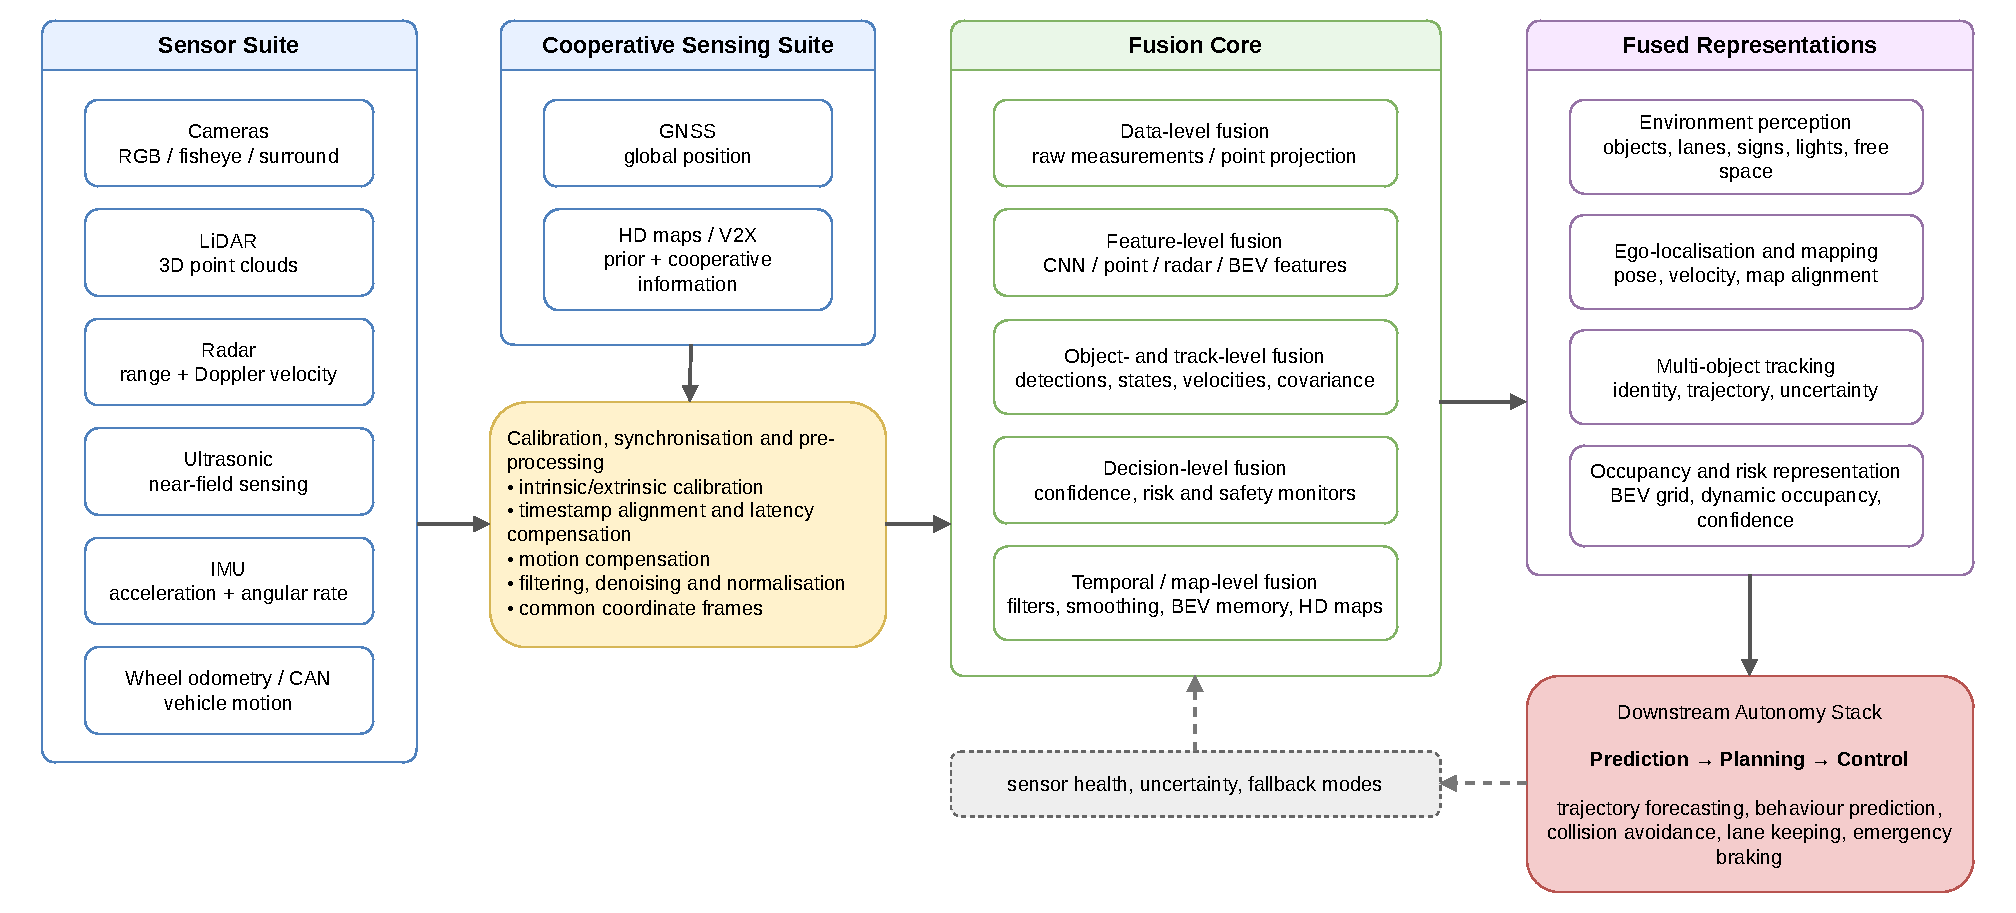
\includegraphics[width=\textwidth]{figures/autonomous_driving_fusion_pipeline.pdf}
    \caption{Autonomous-driving sensor fusion pipeline. Heterogeneous sensor measurements are calibrated, synchronised, and pre-processed before being fused at data, feature, object, decision, temporal, and map levels. The fused representations support environment perception, ego-localisation, mapping, tracking, occupancy estimation, prediction, planning, and control.}
    \label{fig:autonomous-driving-fusion-pipeline}
\end{figure}

Data-level fusion combines low-level measurements directly, for example by projecting LiDAR points into the image plane, aggregating multiple LiDAR sweeps, or associating radar detections with point-cloud clusters. Feature-level fusion combines extracted or learned representations, as in camera--LiDAR, camera--radar, LiDAR--radar, and bird's-eye-view neural architectures\added{, that is, the \emph{multimodal fusion} networks of Chapter~\ref{sec:learning}}. Object- and track-level fusion combines detections, bounding boxes, velocities, class probabilities, covariances, and track states across sensors. Decision-level fusion combines classifier outputs, risk scores, occupancy decisions, or safety-monitoring signals. Temporal fusion uses filtering, smoothing, recurrent networks, temporal attention, or memory-based BEV representations to integrate information over time. Map-level fusion aligns online sensor observations with high-definition maps or previously built local maps.

This layered view clarifies why autonomous driving is a demanding fusion problem. The vehicle must combine onboard exteroceptive sensing for environment perception, proprioceptive sensing for ego-motion estimation, global and map-based references for localisation, and cooperative information for extended situational awareness \cite{2023:IEEE_ITSM,TANG2023109165}. These inputs must then be transformed into representations that are useful for downstream prediction, planning, and control. Errors in calibration, synchronisation, data association, uncertainty modelling, or sensor reliability estimation can therefore propagate through the entire autonomy stack.

\subsection{Spatial Alignment: Extrinsic Calibration and Projection}
\label{subsec:spatial-alignment}

All fusion operations presuppose that the measurements of different sensors are expressed in a common coordinate frame. Each sensor $S$ has its own frame, and the rigid-body pose of that frame with respect to the vehicle (body) frame $V$ is the \emph{extrinsic calibration}
\begin{equation}
\mathbf{T}_{V\!S}=
\begin{bmatrix}
\mathbf{R}_{V\!S} & \mathbf{t}_{V\!S}\\
\mathbf{0}^{\mathsf T} & 1
\end{bmatrix}\in SE(3),
\qquad
\mathbf{R}_{V\!S}\in SO(3),\ \mathbf{t}_{V\!S}\in\mathbb{R}^{3},
\label{eq:extrinsic-se3}
\end{equation}
which maps a point $\mathbf{p}^{S}$ measured in the sensor frame to $\mathbf{p}^{V}=\mathbf{R}_{V\!S}\mathbf{p}^{S}+\mathbf{t}_{V\!S}$, or, in homogeneous coordinates, $\tilde{\mathbf{p}}^{V}=\mathbf{T}_{V\!S}\tilde{\mathbf{p}}^{S}$ with $\tilde{\mathbf{p}}=[\mathbf{p}^{\mathsf T}\ 1]^{\mathsf T}$. Transforms compose by matrix multiplication, so a LiDAR point is expressed in the camera frame through the vehicle frame as $\mathbf{T}_{C\!L}=\mathbf{T}_{V\!C}^{-1}\mathbf{T}_{V\!L}$, and in a world (map) frame $W$ through the ego pose as $\mathbf{T}_{W\!L}(t)=\mathbf{T}_{W\!V}(t)\,\mathbf{T}_{V\!L}$. The collection of such pairwise transforms, with the vehicle frame as the root, is the \emph{transform tree} maintained by the middleware (Section~\ref{subsec:middleware}). Small rotation errors $\delta\boldsymbol{\theta}$ are conveniently written as $\mathbf{R}\approx(\mathbf{I}+[\delta\boldsymbol{\theta}]_{\times})\mathbf{R}$, where $[\cdot]_{\times}$ is the skew-symmetric matrix of the cross product, which is the linearisation used both by calibration estimators and by the error analysis of Section~\ref{subsec:calibration-errors}; a self-contained treatment of $SE(3)$ for estimation is given in \cite{barfoot2017_state_estimation,sola2018_microlie}.

The camera adds an \emph{intrinsic} model. With the pinhole model and a point $\mathbf{p}^{C}=[X\ Y\ Z]^{\mathsf T}$ in the camera frame, the pixel coordinates $(u,v)$ satisfy
\begin{equation}
s\begin{bmatrix}u\\ v\\ 1\end{bmatrix}
=\mathbf{K}\,[\mathbf{R}_{C\!L}\ |\ \mathbf{t}_{C\!L}]\,\tilde{\mathbf{p}}^{L},
\qquad
\mathbf{K}=
\begin{bmatrix}
f_{x} & 0 & c_{x}\\
0 & f_{y} & c_{y}\\
0 & 0 & 1
\end{bmatrix},
\label{eq:lidar-to-image}
\end{equation}
with $s=Z$ the depth of the point, $f_{x},f_{y}$ the focal lengths in pixels and $(c_{x},c_{y})$ the principal point; lens distortion is applied to the normalised coordinates $(X/Z,Y/Z)$ before multiplication by $\mathbf{K}$ \cite{zhang2000_calibration}. Equation~\eqref{eq:lidar-to-image} is the operation behind data-level camera--LiDAR fusion: every LiDAR return with $Z>0$ that falls inside the image is given the colour, the semantic label or the learned feature of the pixel it projects to, and conversely image detections can be lifted to 3D by the LiDAR depth of the pixels they contain (Chapter~\ref{sec:learning}). The extrinsic parameters are estimated offline from a calibration target observed by both sensors \cite{geiger2012_calibration} and must be monitored online, because mounting brackets flex, temperature changes the optics and minor collisions move the sensors; such \emph{calibration drift} is among the open problems of Chapter~\ref{sec:open-challenges}.

\subsection{Temporal Alignment, Ego-Motion Compensation, and Delayed Measurements}
\label{subsec:temporal-alignment}

Sensors sample at different rates and instants, so a second alignment is needed in time. Every measurement carries a timestamp, ideally taken by hardware at the instant of exposure or of the laser pulse and expressed in a common clock (Section~\ref{subsec:middleware}). To relate a measurement taken at time $\tau$ to the ego pose, which is only available at the filter instants $t_{a}\le\tau\le t_{b}$, the pose is interpolated: the position linearly,
\begin{equation}
\mathbf{p}(\tau)=\mathbf{p}(t_{a})+\alpha\,[\mathbf{p}(t_{b})-\mathbf{p}(t_{a})],\qquad \alpha=\frac{\tau-t_{a}}{t_{b}-t_{a}},
\label{eq:pose-interp-pos}
\end{equation}
and the rotation along the geodesic of $SO(3)$,
\begin{equation}
\mathbf{R}(\tau)=\mathbf{R}(t_{a})\,\exp\!\big(\alpha\,\log(\mathbf{R}(t_{a})^{\mathsf T}\mathbf{R}(t_{b}))\big),
\label{eq:pose-interp-rot}
\end{equation}
where $\exp$ and $\log$ are the matrix exponential and logarithm of $SO(3)$ (equivalently, spherical linear interpolation of the corresponding quaternions). At vehicle dynamics the linear interpolation error is negligible for intervals of 10\,ms, but not for the 100\,ms between two LiDAR sweeps.

A rotating LiDAR does not measure a point cloud at one instant: the points of one sweep are acquired over the sweep period $T_{\mathrm{s}}$ (typically $100$\,ms at $10$\,Hz) while the vehicle moves. A point $\mathbf{p}_{i}^{L}$ acquired at time $t_{i}\in[t_{0},t_{0}+T_{\mathrm{s}}]$ is expressed in the vehicle frame at the sweep reference time $t_{0}$ by
\begin{equation}
\mathbf{p}_{i}^{V(t_{0})}=\mathbf{T}_{V(t_{0})V(t_{i})}\,\mathbf{T}_{V\!L}\,\tilde{\mathbf{p}}_{i}^{L},
\qquad
\mathbf{T}_{V(t_{0})V(t_{i})}=\mathbf{T}_{W\!V}(t_{0})^{-1}\mathbf{T}_{W\!V}(t_{i}),
\label{eq:motion-compensation}
\end{equation}
where the relative ego motion $\mathbf{T}_{W\!V}(t_{i})$ is obtained by interpolating the high-rate IMU--odometry prediction of the localisation filter with \eqref{eq:pose-interp-pos}--\eqref{eq:pose-interp-rot}. Without this \emph{ego-motion compensation} (also called de-skewing or motion distortion correction), a vehicle travelling at $25$\,m/s displaces the first and the last point of the same sweep by $2.5$\,m, and a yaw rate of $0.3$\,rad/s rotates them by $1.7^{\circ}$, i.e. by $1.5$\,m laterally at $50$\,m range; the resulting distortions corrupt scan matching, object extents and the camera--LiDAR projection \eqref{eq:lidar-to-image} alike. LiDAR odometry methods such as LOAM perform this correction as part of the registration itself \cite{zhang2014_loam,xu2022_fastlio2}.

Latency produces a related problem at the level of the fusion filter. A camera detection that reaches the tracker $80$\,ms after exposure refers to the state at $t_{k}-80$\,ms, not at $t_{k}$: it is a \emph{delayed} or, if a more recent radar measurement has already been processed, an \emph{out-of-sequence} measurement (OOSM). Ignoring the delay biases the estimate by the motion during the delay, which at a relative speed of $30$\,m/s is $2.4$\,m. The exact treatment keeps a short buffer of past states, covariances and measurements, rolls the filter back to the measurement time $t_{m}$, applies the update there with the stored prediction $\widehat{\mathbf{x}}_{m|m-1}$ and $\mathbf{P}_{m|m-1}$, and re-propagates all later measurements; its cost is proportional to the number of buffered steps. An algebraic alternative retrodicts the current estimate to $t_{m}$ and updates it in a single step, exactly for a one-step lag and approximately for longer lags \cite{barshalom2002_oosm,barshalom2001_estimation}. In both cases the innovation is formed against the state \emph{at the measurement time}, $\boldsymbol{\nu}=\mathbf{y}_{m}-\mathbf{g}(\widehat{\mathbf{x}}_{m|k})$, and not against the current state, which is the single most common timing error in practical trackers. Measurements older than a configured maximum lag are discarded.

\subsection{Effect of Calibration and Synchronisation Errors on Fusion}
\label{subsec:calibration-errors}

Alignment errors are systematic: they do not average out over time and they are not represented in the covariances $\mathbf{R}$ of the individual sensors, so they violate the assumptions behind every fusion rule of Chapter~\ref{sec:classicalSF}. Their effect can be quantified with the linearisation of \eqref{eq:extrinsic-se3}. A yaw (rotation about the vertical axis) error $\delta\psi$ in the extrinsic calibration of a sensor displaces a target at range $r$ laterally by
\begin{equation}
\Delta y \approx r\,\delta\psi,
\label{eq:yaw-error-lateral}
\end{equation}
so a $0.5^{\circ}$ error ($8.7$\,mrad) moves a target at $60$\,m by $0.52$\,m, i.e. by a large fraction of a lane width and by more than the lateral $1\sigma$ accuracy of either sensor in Example~\ref{ex:camera-radar-ci}, whereas at $10$\,m the same error produces only $0.09$\,m. In the image, the same yaw error shifts every projected LiDAR point by $\Delta u\approx f_{x}\,\delta\psi$, i.e. by $8.7$ pixels for $f_{x}=1000$\,pixels, independently of the range, which is why camera--LiDAR misalignment is visible as a constant offset at object boundaries. A translation error $\delta\mathbf{t}$, by contrast, adds a constant offset that does not grow with range, and is therefore less harmful for distant objects but critical for near-field manoeuvring. A time offset $\delta t$ between two sensors is equivalent to a position error $\mathbf{v}_{\mathrm{rel}}\,\delta t$ along the relative velocity: $20$\,ms at $25$\,m/s is $0.5$\,m for a static obstacle and $1.0$\,m for an oncoming vehicle.

The consequences for fusion are threefold. Associations fail: a lateral offset of $0.5$\,m against a fused lateral standard deviation of $0.2$\,m gives a normalised distance of $2.5\sigma$, so the gate \eqref{eq:mahalanobis_gate} starts rejecting correct associations and duplicate tracks appear. Estimates become biased and the filter inconsistent: the NIS \eqref{eq:nis} grows persistently rather than transiently, which is the signature that distinguishes a calibration error from the model mismatch of Example~\ref{ex:ekf-radar-cutin}. Finally, errors that are common to two sensors, for instance the ego-pose used to express both in the map frame, are \emph{correlated} and are double-counted by independent fusion; Example~\ref{ex:camera-radar-ci} quantifies this effect and shows how covariance intersection protects against it. The practical response is to monitor alignment online, by cross-modal consistency statistics and by estimating small calibration corrections as slowly varying states, in the same way as the sensor biases of Example~\ref{ex:gnss-imu-odom}.

\section{Core Fusion Tasks}

Autonomous-driving fusion supports several core tasks. The first is environment perception, where cameras, LiDAR, radar, and maps are used to estimate drivable space, lanes, road boundaries, traffic signs, traffic lights, vehicles, cyclists, pedestrians, and other obstacles. LiDAR depth can improve the spatial accuracy of image-based segmentation, while image semantics can improve the interpretation of sparse point clouds. Radar can contribute long-range range-rate information, especially for moving objects and adverse-weather scenarios. Map priors can further help distinguish valid road areas, pavements, junctions, and lane-level structure.

A second major task is three-dimensional object detection and tracking. Camera--LiDAR fusion is widely used for accurate 3D bounding-box estimation and classification, while radar is valuable for long-range detection and velocity estimation. Tracking extends detection over time by maintaining object identity, position, velocity, acceleration, heading, and uncertainty. Classical filters, smoothing methods, data-association algorithms, and track-management logic remain important even when the detections themselves are produced by deep neural networks.

A third task is ego-localisation and mapping. GNSS, IMU, wheel odometry, cameras, LiDAR, and high-definition maps are fused to estimate the vehicle's position and orientation relative to a local map, global frame, or lane-level map. GNSS alone is insufficient in tunnels, dense urban areas, and multipath environments, while inertial and odometry estimates drift over time. Visual, LiDAR, and map-based localisation can correct this drift, but must handle outdated maps, temporary roadworks, changed lane layouts, perceptual aliasing, and localisation uncertainty.

A fourth task is occupancy, free-space, and risk estimation. Instead of representing the scene only as a list of detected objects, occupancy-based fusion estimates which regions of space are free, occupied, unknown, or dynamically occupied. Risk-aware fusion can incorporate object uncertainty, time-to-collision, occlusion regions, road boundaries, predicted future occupancy, and traffic-rule constraints. These representations are especially important for prediction and planning because the planner must act not only on what is detected, but also on what may be hidden, uncertain, or about to enter the vehicle's path.

Robustness is central to all of these tasks. Rain, fog, snow, darkness, glare, dust, road spray, sensor contamination, and unusual traffic behaviour affect modalities differently. Reliability-aware fusion can adjust sensor weights according to environmental conditions and sensor-health indicators, while temporal fusion can reduce transient false positives and improve consistency. However, fusion cannot compensate for all failures. If several modalities degrade simultaneously, or if the scene lies outside the training or design distribution, the fusion system must detect its own uncertainty and support conservative fallback behaviour.

The remainder of this section makes two of these tasks concrete with runnable worked examples in the style of Chapter~\ref{sec:classicalSF}: ego-localisation by GNSS--IMU--wheel-odometry fusion (Example~\ref{ex:gnss-imu-odom}) and object-level camera--radar track fusion (Example~\ref{ex:camera-radar-ci}). Both use the notation of Table~\ref{tab:notation}; the scripts that generate every number and figure are in the companion repository under \repopath{companion\_\allowbreak repo/\allowbreak examples/\allowbreak }, in the folders \repopath{ch05\_\allowbreak gnss\_\allowbreak imu\_\allowbreak odometry\_\allowbreak ekf} and \repopath{ch05\_\allowbreak camera\_\allowbreak radar\_\allowbreak ci\_\allowbreak fusion}.

\subsection{Worked Example: Ego-Localisation by GNSS--IMU--Wheel-Odometry Fusion}
\label{subsec:ex-gnss}

\begin{example}[GNSS--IMU--wheel-odometry fusion through a tunnel]
\label{ex:gnss-imu-odom}
Consider a vehicle driving for $120$\,s at $13$--$15$\,m/s along a route with a long left curve (yaw rate $0.08$\,rad/s between $t=15$ and $35$\,s) and a right curve ($-0.06$\,rad/s between $t=55$ and $70$\,s). A single-frequency GNSS receiver provides horizontal position fixes at $2$\,Hz with a standard deviation of $\sigma_{\mathrm{GNSS}}=1.5$\,m per axis, except between $t=50$ and $75$\,s, when the vehicle crosses a $346$\,m tunnel and no fix is available. A MEMS gyroscope measures the yaw rate at $100$\,Hz with white noise of standard deviation $0.002$\,rad/s per sample and a constant bias $b=10$\,mrad/s ($0.57^{\circ}$/s), \added{an uncalibrated turn-on offset typical of a low-cost MEMS part (the bias instability of Table~\ref{tab:av-sensor-characteristics} describes instead the much smaller in-run variation that remains once such an offset has been estimated),} and the wheel encoders provide the speed at $100$\,Hz with noise $0.05$\,m/s and a scale error $s=+2$\,\% caused by an incorrect tyre radius. The planar unicycle state
\begin{equation}
\mathbf{x}_{k}=
\begin{bmatrix}
p_{x,k} & p_{y,k} & \psi_{k} & b_{k} & s_{k}
\end{bmatrix}^{\mathsf T}
\end{equation}
collects the position in a local east--north frame, the heading, the gyroscope bias and the wheel scale error. The measured inputs $\mathbf{u}_{k}=[v_{m,k}\ \ \omega_{m,k}]^{\mathsf T}$ drive the process model $\mathbf{f}(\cdot)$ of \eqref{eq:bayes_process_model},
\begin{equation}
\begin{aligned}
p_{x,k+1}&=p_{x,k}+T\,\hat v_{k}\cos\psi_{k}, &\qquad \hat v_{k}&=\frac{v_{m,k}}{1+s_{k}},\\
p_{y,k+1}&=p_{y,k}+T\,\hat v_{k}\sin\psi_{k}, &\qquad \psi_{k+1}&=\psi_{k}+T\,(\omega_{m,k}-b_{k}),\\
b_{k+1}&=b_{k}+q_{b,k}, &\qquad s_{k+1}&=s_{k}+q_{s,k},
\end{aligned}
\label{eq:gnss-imu-process}
\end{equation}
with $T=0.01$\,s. The bias and the scale error are modelled as random walks with intensities $10^{-4}$\,rad\,s$^{-1}$/$\sqrt{\mathrm{s}}$ and $10^{-4}/\sqrt{\mathrm{s}}$, and the input noise enters the position and heading through the Jacobian of \eqref{eq:gnss-imu-process} with respect to $\mathbf{u}_{k}$, \added{denoted $\mathbf{G}_{k}$ here and not to be confused with the measurement matrix $\mathbf{G}$ of Table~\ref{tab:notation},} so that $\mathbf{Q}_{k}=\mathbf{G}_{k}\mathbf{W}\mathbf{G}_{k}^{\mathsf T}+\diag(0,0,T\sigma_{\psi}^{2},T\sigma_{b}^{2},T\sigma_{s}^{2})$ with $\mathbf{W}=\diag(0.05^{2},0.002^{2})$. The GNSS measurement model is linear, $\mathbf{y}_{k}=\mathbf{G}\mathbf{x}_{k}+\mathbf{r}_{k}$ with $\mathbf{G}=[\mathbf{I}_{2}\ \ \mathbf{0}_{2\times3}]$ and $\mathbf{R}=\sigma_{\mathrm{GNSS}}^{2}\mathbf{I}_{2}$, and the EKF of Chapter~\ref{sec:classicalSF}, \eqref{eq:kf_state_prediction}--\eqref{eq:kf_cov_update} with the Jacobian $\mathbf{F}_{k}=\partial\mathbf{f}/\partial\mathbf{x}$, is run at the IMU rate with a GNSS update every $50$ steps. The filter is initialised at the first fix with a $2^{\circ}$ heading error, $b_{0}=s_{0}=0$ and $\mathbf{P}_{0}=\diag(1.5^{2},1.5^{2},(5^{\circ})^{2},0.02^{2},0.05^{2})$. For comparison, a three-state filter $[p_{x}\ p_{y}\ \psi]$ that ignores the bias and the scale error is run on the same data; its heading process noise is inflated ($5\times10^{-3}$\,rad/$\sqrt{\mathrm{s}}$ against $10^{-3}$) so that it works acceptably while GNSS is available.

Figure~\ref{fig:gnss-imu-odom} summarises the outcome. While GNSS fixes are available, both filters follow the route, the five-state filter with an RMS position error of $0.60$\,m, well below the $1.5$\,m of a single fix, and the three-state filter with $5.02$\,m, because the uncompensated bias continuously pulls the heading away and GNSS can only correct it slowly. More importantly, in the $45$\,s before the tunnel the five-state filter has \emph{identified} the sensor errors: at the tunnel entrance it estimates $b=10.29\pm1.39$\,mrad/s ($3\sigma$) against a true value of $10.00$\,mrad/s, and $s=2.15\pm0.33$\,\% against $2.00$\,\%. These two states are observable only because the GNSS fixes constrain the integrated effect of the biases on position, which is why the bias uncertainty collapses during the first curve (panel~c): a bias is distinguishable from a true turn only when the position measurements reveal that the heading did not change as the gyroscope claimed.

Inside the tunnel the filter dead-reckons on the compensated sensors. The five-state position error grows to $3.56$\,m at the end of the $25$\,s outage, while the $3\sigma$ radius $3\sqrt{P_{xx}+P_{yy}}$ reported by the filter grows to $11.94$\,m: the error stays inside the bound throughout the run ($100$\,\% of the samples), so the estimate remains \emph{consistent} and downstream modules can trust the covariance they receive. The three-state filter instead drifts to $63.88$\,m with a heading error of $17.3^{\circ}$, and reports a $3\sigma$ radius of only $19.83$\,m; its error lies inside its own bound for only $7.0$\,\% of the samples. Neither filter is wrong about the sensors; the difference is that the second one has no state in which to put the systematic error, so the error accumulates as $vb\tau^{2}/2$ and the covariance, which only knows about white noise, cannot account for it. At re-acquisition the five-state filter converges within $0.52$\,m after $2$\,s and $0.10$\,m after $5$\,s, whereas the three-state filter still shows $8.79$\,m and $4.45$\,m, because a large heading error must be corrected through position fixes before the position itself can be trusted. The consistency of the five-state filter is confirmed by the NIS \eqref{eq:nis} of the GNSS updates, whose mean over the run is $1.80$ against an expected value of $2$, with $95.2$\,\% of the samples inside the two-sided $95$\,\% interval of $\chi^{2}_{2}$.

The lesson is general and applies to every proprioceptive sensor of Table~\ref{tab:av-sensor-characteristics}: what bounds the drift during an outage is not the quality of the IMU alone but the extent to which its systematic errors have been estimated \emph{before} the outage, and the covariance reported during the outage is only credible if those errors are states of the filter. In practice, longer outages are bridged by adding map matching, visual or LiDAR odometry as further corrections, which is the multi-sensor localisation problem of Chapter~\ref{sec:learning}, and a lane-level requirement (an error below about $0.5$\,m) would in this example be lost after roughly $10$\,s without such aid.
\end{example}

\begin{figure}[!t]
\centering
\resizebox{0.99\columnwidth}{!}{
\begin{tikzpicture}
\begin{groupplot}[
    group style={group size=1 by 3, vertical sep=22mm},
    width=0.95\columnwidth,
    scale only axis,
    tick label style={font=\scriptsize},
    label style={font=\scriptsize},
    legend style={font=\scriptsize, draw=none, fill=white, fill opacity=0.85,
                  text opacity=1},
    grid=major,
    grid style={line width=0.2pt, draw=gray!25},
    axis line style={line width=0.5pt},
    tick align=outside,
    title style={font=\scriptsize, yshift=0.5mm},
]
%% ---------------- panel (a): route ----------------
\nextgroupplot[
    height=3.4cm,
    xlabel={east [m]},
    ylabel={north [m]},
    xmin=-50, xmax=1050,
    ymin=-50, ymax=1150,
    legend pos=north west,
    legend cell align=left,
    legend columns=2,
    title={(a) route in the local east--north frame},
    unbounded coords=discard,
]
\addplot[only marks, mark=*, mark size=0.5pt, draw=MeasGrey, fill=MeasGrey]
    table[x=px_gnss, y=py_gnss, col sep=comma] {data/ch05/gnss_imu_odometry.csv};
\addlegendentry{GNSS fixes}
\addplot[TruthBlack, line width=1.0pt]
    table[x=px_true, y=py_true, col sep=comma] {data/ch05/gnss_imu_odometry.csv};
\addlegendentry{ground truth}
\addplot[EkfBlue, line width=0.9pt, densely dashed]
    table[x=px_est, y=py_est, col sep=comma] {data/ch05/gnss_imu_odometry.csv};
\addlegendentry{EKF, bias states}
\addplot[ManoeuvreOrange!80!black, line width=0.9pt, densely dotted]
    table[x=px_est3, y=py_est3, col sep=comma] {data/ch05/gnss_imu_odometry.csv};
\addlegendentry{EKF, no bias states}
\node[anchor=west, font=\scriptsize, text=black!60] at (axis cs:520,530) {tunnel ($50$--$75$\,s)};
\draw[->, >=stealth, gray!70, line width=0.5pt] (axis cs:515,530) -- (axis cs:455,530);

%% ---------------- panel (b): position error ----------------
\nextgroupplot[
    height=2.9cm,
    xlabel={time $t$ [s]},
    ylabel={position error [m]},
    xmin=0, xmax=120,
    ymin=0, ymax=70,
    ytick={0,20,40,60},
    legend pos=north west,
    legend cell align=left,
    legend columns=2,
    title={(b) position error and reported $3\sigma$ radius},
]
\addplot[draw=none, fill=ManoeuvreOrange, fill opacity=0.45, forget plot]
    coordinates {(50,0) (75,0) (75,70) (50,70)} \closedcycle;
\addplot[draw=none, fill=BandGrey, forget plot]
    table[x=t, y=rad3sig, col sep=comma] {data/ch05/gnss_imu_odometry.csv} \closedcycle;
\addplot[EkfBlue, line width=0.8pt]
    table[x=t, y=err, col sep=comma] {data/ch05/gnss_imu_odometry.csv};
\addlegendentry{error, bias states}
\addplot[RevisionRed!70!black, line width=0.8pt, densely dashed]
    table[x=t, y=err_nobias, col sep=comma] {data/ch05/gnss_imu_odometry.csv};
\addlegendentry{error, no bias states}
\addplot[gray!60, line width=0.5pt, densely dotted]
    table[x=t, y=rad3sig_nobias, col sep=comma] {data/ch05/gnss_imu_odometry.csv};
\addlegendentry{$3\sigma$ radius, no bias states}
\node[anchor=south, font=\scriptsize, text=black!70] at (axis cs:62.5,28) {GNSS outage};
\node[anchor=west, font=\scriptsize, text=black!55] at (axis cs:76,14) {$3\sigma$ radius, bias states (grey band)};

%% ---------------- panel (c): gyro bias ----------------
\nextgroupplot[
    height=2.6cm,
    xlabel={time $t$ [s]},
    ylabel={gyro bias $b$ [mrad/s]},
    xmin=0, xmax=120,
    ymin=0, ymax=20,
    ytick={0,5,10,15,20},
    title={(c) gyroscope-bias estimate with $3\sigma$ band (true value $10$\,mrad/s)},
]
\addplot[draw=none, fill=ManoeuvreOrange, fill opacity=0.45, forget plot]
    coordinates {(50,0) (75,0) (75,20) (50,20)} \closedcycle;
\addplot[name path=bu, draw=none, forget plot]
    table[x=t, y expr=\thisrow{b_est_mrad}+\thisrow{b_sig3_mrad}, col sep=comma] {data/ch05/gnss_imu_odometry.csv};
\addplot[name path=bl, draw=none, forget plot]
    table[x=t, y expr=\thisrow{b_est_mrad}-\thisrow{b_sig3_mrad}, col sep=comma] {data/ch05/gnss_imu_odometry.csv};
\addplot[BandGrey, forget plot] fill between[of=bu and bl];
\addplot[draw=gray!70, line width=0.5pt, densely dotted, forget plot]
    coordinates {(0,10) (120,10)};
\addplot[EkfBlue, line width=0.8pt]
    table[x=t, y=b_est_mrad, col sep=comma] {data/ch05/gnss_imu_odometry.csv};
\end{groupplot}
\end{tikzpicture}
}
\caption{GNSS--IMU--wheel-odometry fusion through a $25$\,s GNSS outage (Example~\ref{ex:gnss-imu-odom}). (a)~Route, GNSS fixes and the estimates of the five-state EKF with gyroscope-bias and wheel-scale states and of the three-state EKF without them. (b)~Position error of the two filters, the $3\sigma$ radius $3\sqrt{P_{xx}+P_{yy}}$ reported by each, and the outage (shaded). The five-state error stays inside its bound and recovers within a few fixes; the three-state error leaves its bound almost immediately because the covariance has no term for the uncompensated bias. (c)~The bias estimate converges during the first curve, when GNSS fixes reveal that the heading did not change as the gyroscope claimed, and is frozen (with slowly growing uncertainty) during the outage.}
\label{fig:gnss-imu-odom}
\end{figure}

\subsection{Worked Example: Object-Level Camera--Radar Track Fusion}
\label{subsec:ex-camradar}

\begin{example}[Camera--radar track fusion with and without covariance intersection]
\label{ex:camera-radar-ci}
A camera track and a radar track refer to the same vehicle at range $r=60$\,m and bearing $\theta=10^{\circ}$ to the left, i.e. at $\mathbf{x}=[59.09\ \ 10.42]^{\mathsf T}$\,m in the ego frame of Example~\ref{ex:ekf-radar-cutin} ($x$ forward, $y$ to the left). The monocular camera estimates the bearing with $\sigma_{\theta}=0.2^{\circ}$ but the range only with $\sigma_{r}=15$\,\% of $r$, i.e. $9$\,m; the radar estimates the range with $\sigma_{r}=0.25$\,m but the bearing with $\sigma_{\theta}=1.5^{\circ}$ (Table~\ref{tab:av-sensor-characteristics}). Each local tracker reports its estimate in Cartesian coordinates with the covariance obtained by linearising the polar-to-Cartesian map, $\mathbf{P}_{i}=\mathbf{J}\,\diag(\sigma_{r,i}^{2},\sigma_{\theta,i}^{2})\,\mathbf{J}^{\mathsf T}$ with $\mathbf{J}=\partial(x,y)/\partial(r,\theta)$, as in \eqref{eq:ekf-radar-jacobian}. The resulting standard deviations are listed in Table~\ref{tab:camera-radar-ci}: the camera ellipse is long and thin along the line of sight (semi-axes $9.00$ and $0.21$\,m), the radar ellipse is short and wide across it ($1.57$ and $0.25$\,m), so each sensor is informative exactly where the other is not.

If the two track errors are independent, the information-additive rule \eqref{eq:independent-track-fusion-state} applies and the fused covariance is $\mathbf{P}_{\mathrm{f}}=(\mathbf{P}_{1}^{-1}+\mathbf{P}_{2}^{-1})^{-1}$, with standard deviations of $0.25$\,m longitudinally and $0.21$\,m laterally: the fusion keeps the radar range and the camera bearing, and the trace of the covariance drops from $2.53$\,m$^{2}$ (radar alone) to $0.106$\,m$^{2}$. Covariance intersection \eqref{eq:ci-cov}--\eqref{eq:ci-est} with the trace criterion \eqref{eq:ci-weight} selects $\omega^{\star}=0.449$ and returns $0.34$\,m and $0.31$\,m, a trace of $0.209$\,m$^{2}$: CI pays about a factor of two in variance for not assuming independence, but it still combines the two sensors directionally, because the scalar $\omega$ weights whole information matrices and the camera information is concentrated in the bearing direction where the radar has none.

\begin{table}[!t]
    \centering
    \small
    \caption{Reported standard deviations of the local and fused tracks of Example~\ref{ex:camera-radar-ci} (independent-error case): longitudinal $\sigma_{x}$, lateral $\sigma_{y}$, semi-axes of the $1\sigma$ ellipse, and trace of the covariance.}
    \label{tab:camera-radar-ci}
    \begin{tabular}{lcccccc}
        \hline
        \textbf{Track} & $\sigma_{x}$ [m] & $\sigma_{y}$ [m] & major [m] & minor [m] & $\tr\mathbf{P}$ [m$^{2}$] & $\omega$ \\
        \hline
        Camera & 8.86 & 1.58 & 9.00 & 0.21 & 81.04 & -- \\
        Radar & 0.37 & 1.55 & 1.57 & 0.25 & 2.53 & -- \\
        Naive independent fusion & 0.25 & 0.21 & 0.25 & 0.21 & 0.106 & -- \\
        Covariance intersection & 0.34 & 0.31 & 0.34 & 0.31 & 0.209 & 0.449 \\
        \hline
    \end{tabular}
\end{table}

Why accept this price? In a real vehicle the two tracks are not independent. Both are expressed in the same frame with the same ego-heading estimate, both may have been initialised from a common detection, both may share the map prior or the ego-motion compensation of Section~\ref{subsec:temporal-alignment}. Suppose the ego heading used by both trackers has an error $\delta\psi$ with standard deviation $\sigma_{\psi}$. It displaces both estimates by the same vector $\delta\psi\,\mathbf{u}$ with $\mathbf{u}=[-p_{y}\ \ p_{x}]^{\mathsf T}$, so that each local covariance becomes $\mathbf{P}_{i}+\sigma_{\psi}^{2}\mathbf{u}\mathbf{u}^{\mathsf T}$ and the cross-covariance is $\mathbf{P}_{12}=\sigma_{\psi}^{2}\mathbf{u}\mathbf{u}^{\mathsf T}$. The actual error covariance of any linear fusion $\widehat{\mathbf{x}}_{\mathrm{f}}=\mathbf{W}_{1}\widehat{\mathbf{x}}_{1}+\mathbf{W}_{2}\widehat{\mathbf{x}}_{2}$ is $\mathbf{W}_{1}\mathbf{P}_{1}\mathbf{W}_{1}^{\mathsf T}+\mathbf{W}_{2}\mathbf{P}_{2}\mathbf{W}_{2}^{\mathsf T}+\mathbf{W}_{1}\mathbf{P}_{12}\mathbf{W}_{2}^{\mathsf T}+\mathbf{W}_{2}\mathbf{P}_{12}^{\mathsf T}\mathbf{W}_{1}^{\mathsf T}$, and its consistency can be measured by the expected normalised estimation error squared, $\mathrm{NEES}=\tr(\mathbf{P}_{\mathrm{rep}}^{-1}\mathbf{P}_{\mathrm{act}})$, which equals the state dimension $2$ for an exactly consistent filter and exceeds it for an over-confident one (Section~\ref{subsec:metrics}). Figure~\ref{fig:camera-radar-ci}(c) sweeps $\sigma_{\psi}$ from $0$ to $2^{\circ}$. The naive rule is consistent only at $\sigma_{\psi}=0$; at $\sigma_{\psi}=0.5^{\circ}$, the calibration-error magnitude of Section~\ref{subsec:calibration-errors}, its NEES is $2.18$ and the actual lateral standard deviation is $0.57$\,m against a reported $0.53$\,m; at $1^{\circ}$ the NEES is $2.47$ ($1.11$\,m actual against $0.92$\,m reported) and at $2^{\circ}$ it is $2.78$ ($2.15$\,m against $1.62$\,m). CI adapts its weight ($\omega^{\star}=0.667$ at $0.5^{\circ}$, $0.814$ at $2^{\circ}$) and remains consistent throughout, with a NEES between $1.00$ and $1.13$ and a reported lateral standard deviation that is never smaller than the actual one ($0.67$\,m reported against $0.56$\,m actual at $0.5^{\circ}$). A Monte-Carlo check with $20\,000$ trials at $\sigma_{\psi}=0.5^{\circ}$ reproduces the analytic values ($2.17$ for the naive rule and $1.04$ for CI), and shows that the two fused estimates are in fact almost equally accurate (RMS lateral errors $0.57$ and $0.56$\,m): the difference is not in the estimate but in the honesty of its covariance.

The example thus answers the question of when CI is needed. If the fusion centre knows that the two tracks have never shared information, the independent rule is optimal and CI wastes half the available information. If the tracks share a prior, a process-noise realisation, an ego pose or a calibration, and the cross-covariance is not tracked, the independent rule under-reports its uncertainty by a factor that grows with the shared component, which in turn corrupts the gates \eqref{eq:mahalanobis_gate} of later associations and the risk estimates of the planner. CI, or its known-correlation counterpart \eqref{eq:correlated-track-fusion-state} when $\mathbf{P}_{12}$ can be propagated, is then the appropriate rule, and it is the standard choice when tracks come from independently developed modules, from other vehicles or from roadside units (Chapter~\ref{sec:MAS}).
\end{example}

\begin{figure}[!t]
\centering
\resizebox{0.99\columnwidth}{!}{
\begin{tikzpicture}
\begin{groupplot}[
    group style={group size=1 by 3, vertical sep=20mm},
    width=0.95\columnwidth,
    scale only axis,
    tick label style={font=\scriptsize},
    label style={font=\scriptsize},
    legend style={font=\scriptsize, draw=none, fill=white, fill opacity=0.85,
                  text opacity=1},
    grid=major,
    grid style={line width=0.2pt, draw=gray!25},
    axis line style={line width=0.5pt},
    tick align=outside,
    title style={font=\scriptsize, yshift=0.5mm},
]
%% ---------------- panel (a): all ellipses ----------------
\nextgroupplot[
    height=2.6cm,
    xlabel={longitudinal $p_x$ [m]},
    ylabel={lateral $p_y$ [m]},
    xmin=35, xmax=85,
    ymin=3, ymax=18,
    legend pos=north west,
    legend cell align=left,
    legend columns=4,
    title={(a) $95\,\%$ error ellipses of the local and fused tracks},
]
\addplot[MeasGrey, line width=0.8pt]
    table[x=cam_x, y=cam_y, col sep=comma] {data/ch05/camera_radar_ci_ellipses.csv};
\addlegendentry{camera}
\addplot[ManoeuvreOrange!80!black, line width=0.8pt]
    table[x=rad_x, y=rad_y, col sep=comma] {data/ch05/camera_radar_ci_ellipses.csv};
\addlegendentry{radar}
\addplot[RevisionRed!70!black, line width=0.8pt]
    table[x=naive_x, y=naive_y, col sep=comma] {data/ch05/camera_radar_ci_ellipses.csv};
\addlegendentry{naive}
\addplot[EkfBlue, line width=0.8pt]
    table[x=ci_x, y=ci_y, col sep=comma] {data/ch05/camera_radar_ci_ellipses.csv};
\addlegendentry{CI}
\addplot[only marks, mark=+, mark size=2.5pt, TruthBlack, forget plot]
    coordinates {(59.0885,10.4189)};

%% ---------------- panel (b): zoom ----------------
\nextgroupplot[
    height=2.6cm,
    xlabel={longitudinal $p_x$ [m]},
    ylabel={lateral $p_y$ [m]},
    xmin=57.5, xmax=61.5,
    ymin=9.4, ymax=12.0,
    title={(b) zoom on the radar and fused ellipses (cross: true position)},
]
\addplot[ManoeuvreOrange!80!black, line width=0.8pt]
    table[x=rad_x, y=rad_y, col sep=comma] {data/ch05/camera_radar_ci_ellipses.csv};
\addplot[RevisionRed!70!black, line width=0.8pt]
    table[x=naive_x, y=naive_y, col sep=comma] {data/ch05/camera_radar_ci_ellipses.csv};
\addplot[EkfBlue, line width=0.8pt]
    table[x=ci_x, y=ci_y, col sep=comma] {data/ch05/camera_radar_ci_ellipses.csv};
\addplot[only marks, mark=+, mark size=2.5pt, TruthBlack]
    coordinates {(59.0885,10.4189)};

%% ---------------- panel (c): NEES sweep ----------------
\nextgroupplot[
    height=2.6cm,
    xlabel={standard deviation $\sigma_\psi$ of the shared heading error [deg]},
    ylabel={NEES},
    xmin=0, xmax=2,
    ymin=0.5, ymax=3.2,
    ytick={1,2,3},
    legend pos=north west,
    legend cell align=left,
    legend columns=2,
    title={(c) consistency of the fused estimate under a shared error},
]
\addplot[draw=gray!70, line width=0.5pt, densely dotted, forget plot]
    coordinates {(0,2) (2,2)};
\addplot[RevisionRed!70!black, line width=0.8pt]
    table[x=sig_psi_deg, y=nees_naive, col sep=comma] {data/ch05/camera_radar_ci_sweep.csv};
\addlegendentry{naive independent fusion}
\addplot[EkfBlue, line width=0.8pt]
    table[x=sig_psi_deg, y=nees_ci, col sep=comma] {data/ch05/camera_radar_ci_sweep.csv};
\addlegendentry{covariance intersection}
\node[anchor=south west, font=\scriptsize, text=black!55] at (axis cs:1.2,2.02) {consistent iff NEES $\le 2$};
\end{groupplot}
\end{tikzpicture}
}
\caption{Camera--radar track fusion (Example~\ref{ex:camera-radar-ci}). (a)~$95\,\%$ error ellipses of the camera track (long along the line of sight), of the radar track (wide across it), and of the two fused estimates for one realisation of the local errors. (b)~Zoom: the naive fused ellipse is the smallest, the CI ellipse is larger by design. (c)~Expected normalised estimation error squared of the two fused estimates when both tracks share an ego-heading error of standard deviation $\sigma_{\psi}$: the independent rule becomes over-confident as the shared component grows, whereas CI stays below the consistency bound at the price of a conservative covariance.}
\label{fig:camera-radar-ci}
\end{figure}

\subsection{Design Guidelines}
\label{subsec:design-guidelines}

The two examples and the alignment analysis of Section~\ref{subsec:temporal-alignment} suggest a small number of rules that recur in practical autonomous-driving fusion systems.
\begin{list4a}
\item Put systematic sensor errors (biases, scale factors, small calibration corrections, clock offsets) into the state vector whenever they are observable; this is what makes covariances credible during outages (Example~\ref{ex:gnss-imu-odom}).
\item Express all measurement uncertainties in the sensor's native coordinates and transform them with the Jacobian, so that the directional structure of each sensor is preserved; fusion exploits complementarity only through that structure (Example~\ref{ex:camera-radar-ci}).
\item Timestamp at acquisition, predict every estimate to a common time before fusing, and form innovations against the state at the measurement time, never against the latest state (Section~\ref{subsec:temporal-alignment}).
\item Use the independent fusion rule only when independence is guaranteed by construction; otherwise propagate the cross-covariance or use covariance intersection, especially across modules, vehicles and infrastructure (Chapter~\ref{sec:MAS}).
\item Monitor the NIS and NEES statistics, the innovation mean and the cross-modal residuals online; persistent inconsistency is the earliest observable symptom of calibration drift, sensor degradation or model mismatch (Chapters~\ref{sec:classicalSF} and~\ref{sec:open-challenges}).
\item Design the sensor layout so that every sector is covered by at least two modalities with different failure modes, and define explicitly what the fusion output is when one of them is unavailable (Section~\ref{subsec:placement}).
\item Prefer learned components where semantics or appearance matter and classical estimators where consistency, interpretability and certification matter; hybrid architectures (Chapter~\ref{sec:learning}) combine both.
\end{list4a}

\section{Datasets, Metrics, and Evaluation}

Public datasets have played a major role in autonomous-driving fusion research. Common benchmarks include KITTI, nuScenes, Waymo Open Dataset, Argoverse, Lyft Level 5, ApolloScape, Oxford RobotCar, Cityscapes, A2D2, ONCE, and BDD100K~\cite{geiger2013_kitti,caesar2020_nuscenes,sun2020_waymo,chang2019_argoverse,cordts2016_cityscapes,yu2020_bdd100k}. These datasets differ in sensor suite, geographic coverage, weather diversity, annotation type, object classes, and supported tasks. A method developed on a camera--LiDAR dataset may not transfer directly to radar fusion, adverse-weather perception, infrastructure-assisted sensing, or map-based localisation. Because the datasets named above are dominated by clear-weather scenes, adverse-condition and robustness-oriented benchmarks are increasingly necessary complements: the Seeing Through Fog dataset provides camera--LiDAR--radar recordings in fog, rain, and snow \cite{bijelic2020_stf}, while corruption suites in the style of RoboBEV systematically perturb inputs to probe how BEV fusion architectures degrade \cite{dong2023_robobev}. For a \deleted{survey}\added{book} whose central claim is robustness through fusion, such benchmarks matter more than average-case leaderboards. % [July 2026 pass] Dataset name-dropping without citations was a reviewer-visible gap; added citations and an adverse-weather benchmark note. Bib entries in references_additions.bib.

Table~\ref{tab:av-datasets} summarises the public datasets most used for fusion research. Three remarks help in reading it. The sensor column decides which fusion problems a dataset can support at all: only nuScenes, Waymo Open, Argoverse~2 (through its lidar and sensor splits), ONCE, A2D2 and the adverse-weather sets record radar or a full surround camera--LiDAR rig with synchronised timestamps and calibrations, while KITTI, Cityscapes and BDD100K are essentially camera or camera--LiDAR datasets. The scale column should be compared with the number of \emph{distinct} scenes rather than of frames, because consecutive frames of a $20$\,s sequence are highly correlated. The conditions column explains why robustness studies need the last rows: the large benchmarks are recorded mostly in daylight and clear weather, so a method that leads their leaderboards has not been tested where fusion is supposed to pay off.

\begin{table}[!t]
    \centering
    \scriptsize
    \caption{Public datasets commonly used in autonomous-driving fusion research (indicative figures taken from the respective publications; ``scenes'' are driving segments of typically $8$--$20$\,s).}
    \label{tab:av-datasets}
    \begin{tabular}{>{\raggedright\arraybackslash}p{0.14\linewidth} >{\raggedright\arraybackslash}p{0.05\linewidth} >{\raggedright\arraybackslash}p{0.23\linewidth} >{\raggedright\arraybackslash}p{0.17\linewidth} >{\raggedright\arraybackslash}p{0.17\linewidth} >{\raggedright\arraybackslash}p{0.14\linewidth}}
        \hline
        \textbf{Dataset} & \textbf{Year} & \textbf{Sensors} & \textbf{Scale} & \textbf{Tasks} & \textbf{Conditions} \\
        \hline
        KITTI \cite{geiger2013_kitti} & 2012 & 2 stereo pairs, 64-layer LiDAR, GNSS/IMU & 22 odometry sequences, 15k annotated frames & 2D/3D detection, tracking, odometry, stereo, flow & Daytime, clear, one city \\
        \hline
        Cityscapes \cite{cordts2016_cityscapes} & 2016 & Stereo camera & 5k fine and 20k coarse annotated images, 50 cities & Semantic and instance segmentation & Daytime, fair weather \\
        \hline
        Oxford RobotCar \cite{maddern2017_robotcar} & 2017 & Stereo and mono cameras, 2D/3D LiDAR, GNSS/INS & 100+ traversals of a 10\,km route over one year & Localisation, mapping, long-term change & All seasons, rain, snow, night \\
        \hline
        Argoverse 1 \cite{chang2019_argoverse} & 2019 & 7 ring cameras, 2 stereo, 2 LiDARs, HD map & 113 scenes (3D tracking), 324k trajectories (forecasting) & 3D tracking, motion forecasting, map-based tasks & Two cities, day and some night \\
        \hline
        nuScenes \cite{caesar2020_nuscenes} & 2019 & 6 cameras, 32-layer LiDAR, 5 radars, GNSS/IMU & 1000 scenes, 1.4M images, 390k LiDAR sweeps, 1.4M boxes & 3D detection, tracking, prediction, occupancy (extensions) & Boston and Singapore, rain and night included \\
        \hline
        Waymo Open \cite{sun2020_waymo} & 2019 & 5 cameras, 5 LiDARs & 1150 scenes, 12M 3D boxes & 2D/3D detection, tracking, domain adaptation, motion & Several US cities, day, night, rain \\
        \hline
        A2D2 \cite{geyer2020_a2d2} & 2020 & 6 cameras, 5 LiDARs, bus data & 41k annotated frames, 390k unannotated & Semantic segmentation, 3D boxes, point-cloud tasks & Southern Germany, daytime \\
        \hline
        BDD100K \cite{yu2020_bdd100k} & 2020 & Mono camera, GNSS/IMU & 100k videos, 10 tasks & 2D detection, segmentation, tracking, lane & Diverse weather and time of day, US \\
        \hline
        Seeing Through Fog \cite{bijelic2020_stf} & 2020 & Stereo and gated cameras, LiDAR, radar, FIR camera & \deleted{12k clear and 1.5k adverse-weather frames}\added{12k real-world samples in mixed weather, 1.5k fog-chamber samples}, 10k\,km & 3D detection under adverse weather & Fog, rain, snow, night, Northern Europe \\
        \hline
        RADIATE \cite{sheeny2021_radiate} & 2021 & Scanning radar, LiDAR, stereo camera, GNSS/IMU & 3\,h, 200k radar objects & Radar-based detection and tracking in bad weather & Fog, rain, snow, night \\
        \hline
        ONCE \cite{mao2021_once} & 2021 & 7 cameras, 40-layer LiDAR & 1M LiDAR frames, 7M images, 15k annotated & 3D detection, semi/self-supervised learning & Chinese cities, day and night, rain \\
        \hline
        Argoverse 2 \cite{wilson2021_argoverse2} & 2021 & 7 ring cameras, 2 stereo, 2 LiDARs, HD map & 1000 sensor scenes, 20k lidar scenes, 250k forecasting scenarios & 3D detection, tracking, forecasting, map tasks & Six US cities, varied time of day and weather \\
        \hline
    \end{tabular}
\end{table}

Fusion systems can be evaluated across 2D object detection, 3D object detection, semantic segmentation, panoptic segmentation, lane detection, free-space estimation, multi-object tracking, ego-localisation, odometry, mapping, occupancy prediction, and trajectory prediction. Detection tasks commonly use average precision and mean average precision, while segmentation tasks use intersection-over-union and mean intersection-over-union. Localisation and odometry are often evaluated using absolute trajectory error, relative pose error, drift, heading error, and map-matching accuracy. Tracking metrics additionally assess identity switches, track fragmentation, missed detections, false positives, and trajectory consistency. Section~\ref{subsec:metrics} gives the definitions of the metrics named here.

\subsection{Metric Definitions}
\label{subsec:metrics}

Detection metrics start from the classification of each prediction as a true positive (TP), a false positive (FP) or, for each unmatched ground-truth object, a false negative (FN), where a match is decided by an overlap or distance criterion. Precision and recall, $\mathrm{P}=\mathrm{TP}/(\mathrm{TP}+\mathrm{FP})$ and $\mathrm{R}=\mathrm{TP}/(\mathrm{TP}+\mathrm{FN})$, are computed as the confidence threshold is lowered, and the average precision is the area under the resulting precision--recall curve,
\begin{equation}
\mathrm{AP}=\int_{0}^{1}\tilde{p}(r)\,\mathrm{d}r,\qquad \tilde{p}(r)=\max_{r'\ge r}p(r'),
\label{eq:ap}
\end{equation}
where the interpolation $\tilde{p}$ makes the curve monotone \cite{everingham2010_voc}; mAP averages AP over classes and, in COCO style, over a set of overlap thresholds \cite{lin2014_coco}. The overlap criterion for boxes and for segmentation masks is the intersection over union,
\begin{equation}
\mathrm{IoU}(A,B)=\frac{|A\cap B|}{|A\cup B|},\qquad
\mathrm{mIoU}=\frac{1}{C}\sum_{c=1}^{C}\frac{\mathrm{TP}_{c}}{\mathrm{TP}_{c}+\mathrm{FP}_{c}+\mathrm{FN}_{c}},
\label{eq:iou}
\end{equation}
with the second expression computed over pixels (or voxels) of class $c$. In 3D the IoU is sensitive to small orientation and extent errors of distant objects, which is why nuScenes matches detections by the Euclidean distance between box centres on the ground plane, with thresholds of $0.5$, $1$, $2$ and $4$\,m, averages AP over these thresholds and over ten classes, and complements the resulting mAP with five true-positive error metrics, the mean average translation, scale, orientation, velocity and attribute errors (mATE, mASE, mAOE, mAVE, mAAE), combined into the nuScenes detection score
\begin{equation}
\mathrm{NDS}=\frac{1}{10}\Big[5\,\mathrm{mAP}+\sum_{m\in\{\mathrm{mATE},\mathrm{mASE},\mathrm{mAOE},\mathrm{mAVE},\mathrm{mAAE}\}}\big(1-\min(1,m)\big)\Big]
\label{eq:nds}
\end{equation}
\cite{caesar2020_nuscenes}. The composition of \eqref{eq:nds} matters for fusion: half of the score rewards finding the objects, the other half rewards estimating their state, and the velocity term in particular is where radar fusion shows its value \cite{nabati2021_centerfusion,kim2023_crn}.

Multi-object tracking adds identity. The CLEAR MOT accuracy
\begin{equation}
\mathrm{MOTA}=1-\frac{\sum_{t}\big(\mathrm{FN}_{t}+\mathrm{FP}_{t}+\mathrm{IDS}_{t}\big)}{\sum_{t}\mathrm{GT}_{t}}
\label{eq:mota}
\end{equation}
counts missed objects, false alarms and identity switches (IDS) relative to the number of ground-truth objects over all frames, and MOTP measures the localisation precision of the matched pairs \cite{bernardin2008_clearmot}. Because MOTA is evaluated at a single confidence threshold, the 3D tracking benchmarks use its average over recall levels: with $\mathrm{MOTAR}_{r}=\max\{0,\,1-[\mathrm{FP}_{r}+\mathrm{FN}_{r}+\mathrm{IDS}_{r}-(1-r)\,\mathrm{GT}]/(r\,\mathrm{GT})\}$ the recall-normalised accuracy at recall $r$,
\begin{equation}
\mathrm{AMOTA}=\frac{1}{n}\sum_{r\in\{\frac{1}{n},\frac{2}{n},\dots,1\}}\mathrm{MOTAR}_{r},
\label{eq:amota}
\end{equation}
and AMOTP is defined analogously from the localisation error \cite{weng2020_ab3dmot,caesar2020_nuscenes}.

Odometry and localisation are evaluated on trajectories. Given estimated poses $\mathbf{T}_{i}$ and ground-truth poses $\mathbf{T}_{i}^{\star}$ in $SE(3)$, aligned by a single rigid (or similarity) transform $\mathbf{S}$ when the estimate lives in an arbitrary frame, the absolute trajectory error and the relative pose error over a horizon $\Delta$ are
\begin{equation}
\mathrm{ATE}=\sqrt{\frac{1}{N}\sum_{i=1}^{N}\big\|\mathrm{trans}\big(\mathbf{T}_{i}^{\star-1}\,\mathbf{S}\,\mathbf{T}_{i}\big)\big\|^{2}},
\qquad
\mathbf{E}_{i}^{\Delta}=\big(\mathbf{T}_{i}^{\star-1}\mathbf{T}_{i+\Delta}^{\star}\big)^{-1}\big(\mathbf{T}_{i}^{-1}\mathbf{T}_{i+\Delta}\big),
\label{eq:ate-rpe}
\end{equation}
with the RPE given by the RMS of the translational (and separately the rotational) part of $\mathbf{E}_{i}^{\Delta}$ \cite{sturm2012_rgbd}. ATE measures global consistency and is dominated by drift and loop-closure quality; RPE measures local accuracy and is the appropriate metric for the dead-reckoning segments of Example~\ref{ex:gnss-imu-odom}. The KITTI odometry benchmark reports the RPE as a translational drift in percent and a rotational drift in degrees per metre, averaged over segments of $100$--$800$\,m \cite{geiger2013_kitti}.

Filter consistency is evaluated with the normalised estimation error squared,
\begin{equation}
\epsilon_{k}=(\mathbf{x}_{k}-\widehat{\mathbf{x}}_{k|k})^{\mathsf T}\mathbf{P}_{k|k}^{-1}(\mathbf{x}_{k}-\widehat{\mathbf{x}}_{k|k}),
\qquad
\mathbb{E}[\epsilon_{k}]=n_{x},
\label{eq:nees}
\end{equation}
which under the linear--Gaussian assumptions is $\chi^{2}_{n_{x}}$-distributed; averaged over $M$ Monte-Carlo runs, $M\bar{\epsilon}_{k}\sim\chi^{2}_{Mn_{x}}$, so that a two-sided $95$\,\% acceptance region can be tested at every time step \cite{barshalom2001_estimation}. The NEES requires ground truth and is therefore an offline, dataset-based metric; its online counterpart is the NIS \eqref{eq:nis} of Chapter~\ref{sec:classicalSF}, which replaces the unknown state error by the innovation and is what the vehicle can monitor at run time. Example~\ref{ex:gnss-imu-odom} reports both, and Example~\ref{ex:camera-radar-ci} uses the expected NEES $\tr(\mathbf{P}_{\mathrm{rep}}^{-1}\mathbf{P}_{\mathrm{act}})$ to compare fusion rules. For learned components that output class probabilities, the analogous question is whether a confidence of $0.9$ is correct $90$\,\% of the time; the expected calibration error bins the $N$ predictions by confidence and measures
\begin{equation}
\mathrm{ECE}=\sum_{m=1}^{M}\frac{|B_{m}|}{N}\,\big|\mathrm{acc}(B_{m})-\mathrm{conf}(B_{m})\big|,
\label{eq:ece-metric}
\end{equation}
where $\mathrm{acc}(B_{m})$ and $\mathrm{conf}(B_{m})$ are the empirical accuracy and the mean confidence in bin $B_{m}$ \cite{guo2017_calibration}. Deep networks are frequently over-confident, and a decision-level fusion that treats their scores as probabilities inherits this miscalibration exactly as an independent track fusion inherits an under-reported covariance (Chapter~\ref{sec:learning}).

For autonomous driving, average benchmark accuracy is not sufficient. Evaluation should also consider latency, throughput, memory footprint, energy consumption, hardware utilisation, uncertainty calibration, false-negative rates for vulnerable road users, robustness under degraded sensing, and performance in rare safety-critical scenarios. Scenario-based testing, simulation, hardware-in-the-loop evaluation, closed-course testing, and real-world trials are important complements to public benchmarks because many critical failures are rare, context-dependent, and difficult to capture in static datasets.

Scenario-based evaluation formalises this complement. A \emph{scenario} is a parametrised description of a traffic situation (a cut-in at a given relative speed and gap, a pedestrian emerging from occlusion at a given distance, a tunnel exit against low sun), and the evaluation samples the parameter space, in simulation, on closed courses or by re-simulating recorded data, to estimate the failure probability of the fused system as a function of the scenario parameters rather than a single average score \cite{riedmaier2020_scenario}. For fusion, the relevant parameters include the ones that the benchmarks above hold fixed: sensor degradation (fog density, rain rate, soiling, blockage of one modality), calibration and timing errors of the magnitudes discussed in Section~\ref{subsec:calibration-errors}, communication latency for cooperative inputs, and outage durations of the kind simulated in Example~\ref{ex:gnss-imu-odom}. Robustness benchmarks such as RoboBEV \cite{dong2023_robobev} are the dataset-side version of the same idea: they apply controlled corruptions to the inputs of a recorded dataset and report the degradation relative to clean performance, which makes it possible to attribute a loss of accuracy to a specific modality or to the fusion rule. Together with the consistency statistics of Section~\ref{subsec:metrics}, these evaluations provide the evidence needed by the verification and validation processes discussed in Chapter~\ref{sec:open-challenges}.

\section{Implementation and Validation}

A practical autonomous-driving fusion system requires more than the fusion algorithm itself. It also requires sensor drivers, calibration tools, data logging, synchronisation mechanisms, coordinate-frame management, visualisation tools, middleware, and deployment-aware software design. ROS and ROS~2 are widely used for prototyping because they provide modular communication between sensor, perception, localisation, planning, and control nodes. Python is often used for rapid algorithm development and evaluation, while C++ is commonly used for performance-critical deployment. Deep learning frameworks such as PyTorch and TensorFlow are used for training and evaluating learning-based fusion models.

Practical systems must maintain consistent coordinate frames and timestamps throughout the processing pipeline. This typically requires calibration files, transform trees, time-offset estimation, motion compensation, and careful handling of missing, delayed, or out-of-order messages. Deployment platforms may include CPUs, GPUs, FPGAs, and heterogeneous embedded computing architectures. FPGA-based Kalman and LQG implementations illustrate how estimation cores can be accelerated and validated using hardware-in-the-loop frameworks \cite{deliparaschos_fpgabased_2016}. Such implementations are relevant because latency, energy consumption, and timing determinism become critical when fusion outputs directly affect planning and control.

Several implementation patterns illustrate the connection between fusion theory and deployment. GNSS--IMU--wheel odometry fusion uses inertial and odometry measurements for prediction and GNSS or map-based updates for drift correction. Camera--LiDAR feature-level fusion combines semantic image features with geometric point-cloud or BEV features for 3D perception. Radar--camera--LiDAR track-level fusion associates detections across modalities and maintains object states over time. Reliability-aware fusion adapts sensor weights according to visibility, blockage, timestamp delay, calibration quality, detection confidence, environmental condition, and sensor-health indicators. The first and the third of these patterns are the subject of Examples~\ref{ex:gnss-imu-odom} and~\ref{ex:camera-radar-ci}.

\subsection{Latency and Throughput Budget}
\label{subsec:latency}

Fusion sits in the middle of a sensing-to-actuation chain whose total latency determines how far the vehicle travels before it can react to what the sensors saw. Indicative contributions are the sensor acquisition interval (an exposure and read-out of $10$--$30$\,ms for a camera, a full sweep of $100$\,ms for a $10$\,Hz LiDAR), transfer and decoding (a few milliseconds), detection networks ($20$--$60$\,ms on an automotive GPU), fusion and tracking (a few milliseconds for object-level fusion, tens of milliseconds for dense BEV fusion), prediction and planning ($50$--$100$\,ms), the control cycle ($10$--$20$\,ms) and the actuator response ($100$--$300$\,ms for the brake hydraulics). Summing a typical chain gives
\begin{equation}
\tau_{\mathrm{e2e}}=\tau_{\mathrm{sense}}+\tau_{\mathrm{xfer}}+\tau_{\mathrm{detect}}+\tau_{\mathrm{fuse}}+\tau_{\mathrm{plan}}+\tau_{\mathrm{ctrl}}+\tau_{\mathrm{act}}\approx 300\text{--}500\ \mathrm{ms},
\label{eq:latency-budget}
\end{equation}
during which a vehicle at $30$\,m/s travels $9$--$15$\,m. Two consequences follow for the fusion design. First, the fusion module must stamp its output with the time it refers to and, when asked for the current state, predict it forward with the process model, $\widehat{\mathbf{x}}(t_{\mathrm{now}})=\mathbf{f}(\widehat{\mathbf{x}}(t_{\mathrm{meas}}),t_{\mathrm{now}}-t_{\mathrm{meas}})$, with the covariance inflated accordingly; the age of the data is part of the uncertainty. Second, throughput and latency are different budgets: pipelining the stages of \eqref{eq:latency-budget} on several cores keeps up with a $10$\,Hz LiDAR without reducing the age of any individual result, whereas reducing latency requires shortening the critical path, for instance by fusing radar tracks at their native $20$\,Hz without waiting for the slower camera or LiDAR result, which is one argument for asynchronous, sequential-update filters of the kind used in Example~\ref{ex:gnss-imu-odom}. The budget must be met in the worst case rather than on average: jitter in $\tau_{\mathrm{detect}}$ caused by the number of objects in the scene, or a garbage-collection pause in the middleware, is as harmful to a controller as a systematic delay, and worst-case execution times are what certification asks for. Accelerators help where the computation is regular: the FPGA implementations of Kalman and LQG cores in \cite{deliparaschos_fpgabased_2016,deliparaschos_fpga_2016} achieve microsecond-level, cycle-accurate latencies that a general-purpose processor cannot guarantee, at the price of fixed-point arithmetic whose precision must be verified against the floating-point reference (Chapter~\ref{sec:open-challenges}).

\subsection{Middleware, Time Synchronisation, and Transform Trees}
\label{subsec:middleware}

The temporal and spatial alignment of Section~\ref{subsec:temporal-alignment} is implemented in the middleware. In ROS~2 \cite{macenski2022_ros2} every message carries a header with a timestamp and a frame identifier; the publish--subscribe transport over DDS allows the quality of service (reliable or best-effort delivery, history depth, deadlines) to be chosen per topic, so that a high-rate IMU stream can be best-effort while GNSS fixes and object lists are delivered reliably. A common time base is a precondition. Sensors and computers are synchronised by the Precision Time Protocol \cite{ieee1588_2019}, often disciplined by the pulse-per-second output of the GNSS receiver, and cameras are triggered by hardware so that the exposure coincides with the instant at which the LiDAR azimuth points into their field of view; without such triggering the camera--LiDAR offset is a random variable with the consequences quantified in Section~\ref{subsec:calibration-errors}. Software timestamps taken on message reception are not a substitute, because they include the transfer and queueing delays that the fusion is supposed to compensate.

With timestamps available, messages from several sensors are grouped by \emph{approximate-time} synchronisation: a policy that collects, for each sensor, the message whose stamp is closest to a common pivot and emits the set when all stamps lie within a tolerance window, discarding messages that cannot be matched. The tolerance is a design parameter: a window of $10$\,ms at $25$\,m/s corresponds to the $0.25$\,m of unmodelled motion that the fusion must be prepared to absorb in its covariance, and the policy should be bypassed altogether, in favour of sequential updates, when the sensors have very different rates. Spatial alignment is handled by the transform tree, in ROS~2 the \texttt{tf2} library, which stores time-indexed transforms between all frames and answers queries of the form ``$\mathbf{T}_{AB}$ at time $\tau$'' by composing the chain between the two frames and interpolating each link with \eqref{eq:pose-interp-pos}--\eqref{eq:pose-interp-rot}. Static transforms hold the extrinsic calibrations \eqref{eq:extrinsic-se3}; dynamic transforms hold the ego pose published by the localisation filter. The structure makes the frame conventions explicit, but it also centralises a failure mode: a wrong or stale calibration in the tree silently corrupts every consumer. Vehicle-oriented stacks built on this middleware, such as Autoware \cite{kato2018_autoware}, add the real-time executors, the deterministic callback scheduling and the safety monitors that general-purpose ROS~2 does not provide by default.

\subsection{Determinism and Hardware-in-the-Loop Validation}
\label{subsec:hil}

A fusion system is \emph{deterministic} if the same input sequence always produces the same output. Determinism is a prerequisite for debugging, for regression testing and for the reproducible evidence that safety cases require, and it is easily lost: multi-threaded executors process callbacks in an order that depends on the timing of message arrival, floating-point reductions on GPUs are not associative, learned components may use non-deterministic kernels, and approximate-time synchronisation emits different groupings when queues are serviced at different instants. Practical measures are to drive all modules from the message timestamps rather than from the wall clock, to order the processing of buffered measurements by timestamp with explicit handling of out-of-sequence data (Section~\ref{subsec:temporal-alignment}), to pin executors to cores with fixed priorities, and to record all inputs so that any run can be replayed offline and compared bit for bit. The worked examples of this chapter are deterministic in this sense: a fixed random seed makes every number in the text reproducible, and the same discipline applies to a vehicle.

Validation then proceeds through stages that trade realism for controllability. Software-in-the-loop runs the fusion code against simulated sensors in CARLA, AirSim or similar simulators \cite{dosovitskiy_carla_2017,shah_airsim_2017}, which gives ground truth for the metrics of Section~\ref{subsec:metrics} and allows the scenario sweeps of the previous section. Hardware-in-the-loop (HIL) executes the fusion on the target electronic control unit, with the vehicle dynamics and the sensor front-ends emulated in real time by a simulator that injects synthetic raw data, or recorded data with synthetic perturbations, through the real interfaces; it is the only stage at which the latency budget \eqref{eq:latency-budget}, the time synchronisation and the behaviour under dropped or delayed messages can be verified under realistic timing. The FPGA estimation cores of \cite{deliparaschos_fpgabased_2016} were validated in exactly this way, with the plant simulated in real time and the hardware estimator closed in the loop, which is the pattern that the infrastructure described next generalises to complete vehicles and to cooperative, infrastructure-assisted fusion.

System-level validation is essential because real-world fusion performance depends not only on the algorithm, but also on timing, sensor configuration, calibration quality, communication latency, compute resources, and interaction with downstream planning and control. Integrated testing and simulation infrastructures can evaluate sensor fusion components together with perception, control, and human-interaction models \cite{deliparaschos_preliminary_2020}. A concrete example is the Multi-User Environment for Autonomous Vehicle Innovation (MUEAVI), an integrated validation infrastructure for autonomous vehicles and smart-city transport. The facility combines physical road infrastructure, heterogeneous sensor networks, embedded edge processing, a central data-fusion centre, visualisation tools, scenario recording, and software-based validation \cite{deliparaschos_preliminary_2020}.

The MUEAVI camera-tracking pipeline illustrates how infrastructure-level sensing can be connected to perception and actuation through middleware. In this scenario, a full-HD video stream from a PTZ camera is decoded using the NVIDIA DeepStream framework, object detection and tracking are performed, object-detection messages are broadcast through Apache Kafka, and the \texttt{kafka\_ROS\_connector} node converts these messages into custom ROS messages. The \texttt{deepstream\_ptz\_control} node then computes relative pan--tilt--zoom commands from the detected-object list, while the \texttt{ptz\_control} node sends these commands to the PTZ camera and publishes camera status information \cite{deliparaschos_preliminary_2020}. Figure~\ref{fig:mueavi-camera-tracking} illustrates this camera-tracking control-loop validation scenario.

\begin{figure}[!t]
    \centering
    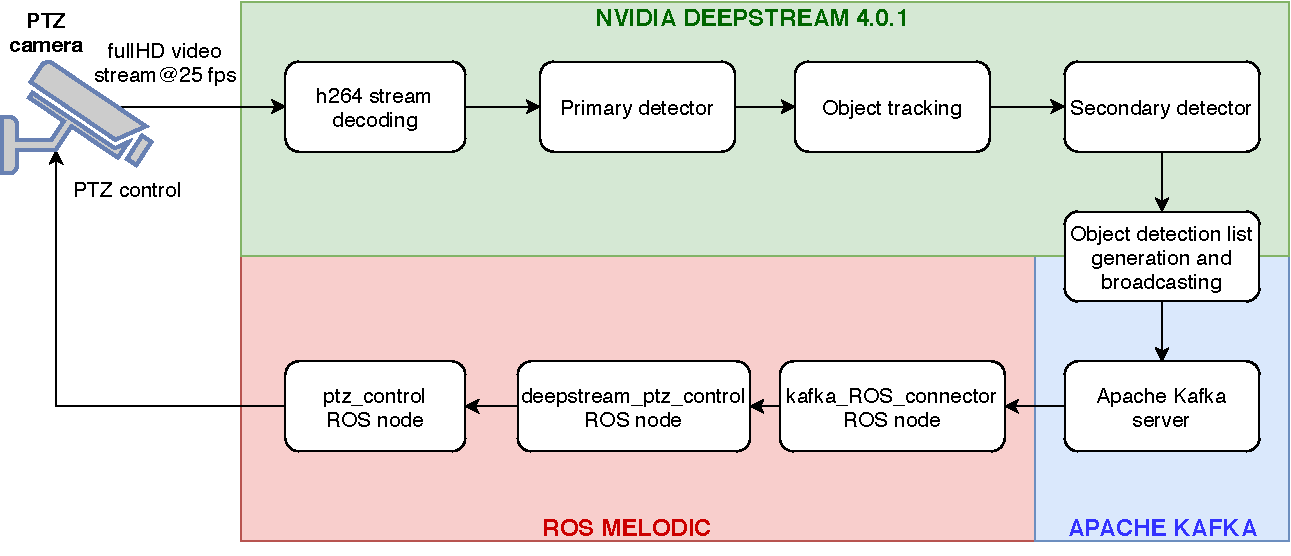
\includegraphics[width=\textwidth]{figures/tracking_with_camera.pdf}
    \caption{Camera tracking control-loop validation scenario based on the MUEAVI infrastructure. The pipeline receives a full-HD video stream from a PTZ camera, decodes it using the NVIDIA DeepStream framework, performs object detection and tracking, broadcasts object-detection messages through Apache Kafka, and converts these messages into ROS messages using the \texttt{kafka\_ROS\_connector} node. The \texttt{deepstream\_ptz\_control} ROS node computes relative pan--tilt--zoom commands from the detected-object list, while the \texttt{ptz\_control} ROS node sends the commands to the PTZ camera and publishes camera status information.}
    \label{fig:mueavi-camera-tracking}
\end{figure}

Infrastructure-supported fusion systems extend this idea by combining data from vehicle-mounted and fixed sensing sources. Roadside cameras, LiDARs, and radars can observe vehicles and vulnerable road users from viewpoints that differ from those available to the ego vehicle. This can improve object tracking, support cooperative perception, provide external validation for onboard perception, and help analyse occluded or safety-critical scenarios.

A representative infrastructure-assisted architecture consists of three layers. The first layer performs local acquisition and preprocessing close to the sensors, including video decoding, timestamping, point-cloud filtering, radar parsing, clustering, and object detection. Camera-based detection can be implemented using real-time neural detectors such as YOLOv3 \cite{redmon_yolov3_2018}. LiDAR and radar preprocessing commonly involves point-cloud filtering, downsampling, segmentation, and clustering, with tools such as the Point Cloud Library and algorithms such as DBSCAN being widely used in practical implementations \cite{rusu_pcl_2011, ester_dbscan_1996}. The second layer performs centralised or distributed fusion, including coordinate transformation, multi-object tracking, object classification, sensor-selection logic, and scenario classification. The third layer supports validation, visualisation, data storage, and comparison against simulation or reference measurements.

This type of architecture connects sensor fusion with verification and validation rather than treating it as an isolated perception module. It also exposes practical implementation issues that are often hidden in algorithm-only descriptions, including time synchronisation, multi-sensor cross-calibration, middleware design, network latency, edge-computing constraints, and real-time data storage. Hardware--software co-design and systematic sensor-selection methods are therefore relevant when fusion algorithms must be deployed on embedded or resource-constrained platforms \cite{deliparaschos_fpga_2016}.

\subsection{Links to the Other Chapters}
\label{subsec:ch05-links}

The material of this chapter instantiates, in one application, the methods of the rest of the book. The alignment steps of Section~\ref{subsec:spatial-alignment} and the two worked examples are classical estimation problems in the sense of Chapter~\ref{sec:classicalSF}: the EKF equations \eqref{eq:kf_state_prediction}--\eqref{eq:kf_cov_update}, the consistency diagnostics \eqref{eq:nis} and the track-fusion rules \eqref{eq:independent-track-fusion-state}--\eqref{eq:ci-weight} are used unchanged. The perception side, in which detections are produced by learned camera--LiDAR--radar networks and BEV or occupancy representations, is the subject of Chapter~\ref{sec:learning}, whose hybrid architectures explain how learned detections feed the classical trackers used here. The cooperative inputs of Table~\ref{tab:av-cooperative-inputs}, the fusion of tracks across vehicles and roadside units, and the consistency problems that motivate covariance intersection in distributed settings are developed in Chapter~\ref{sec:MAS}. Finally, the issues that this chapter can only flag, calibration drift, adverse conditions, real-time embedded deployment, verification and safety assurance, are the open challenges of Chapter~\ref{sec:open-challenges}.

\problemsection

\begin{prob}\label{prob:ch05:1}
A forward camera has focal length $f_{x}=f_{y}=1200$\,pixels and a $1920\times1080$ image. Its extrinsic calibration with respect to the LiDAR has a yaw error of $0.5^{\circ}$. (a)~By how many pixels is a LiDAR point projected through \eqref{eq:lidar-to-image} displaced horizontally, and does the displacement depend on the range? (b)~What lateral position error does the same yaw error produce for an object at $20$\,m and at $80$\,m if the camera bearing is used to position it? (c)~A translation error of $10$\,cm along the camera $x$ axis is present instead: how large is the projected pixel error at $20$\,m and at $80$\,m, and what does this imply for near-field versus far-field fusion?
\end{prob}

\begin{prob}\label{prob:ch05:2}
A camera and a radar are synchronised in software with a residual time offset of $30$\,ms, the ego vehicle drives at $20$\,m/s. (a)~Compute the apparent longitudinal misalignment between the two sensors for a static obstacle and for an oncoming vehicle travelling at $20$\,m/s. (b)~The fused longitudinal standard deviation of the obstacle is $0.3$\,m; compute the normalised distance of the offset in both cases and discuss whether the gate \eqref{eq:mahalanobis_gate} with $\gamma=9.21$ ($99$\,\% for two degrees of freedom) would still associate the two detections. (c)~Propose a state augmentation that would allow the filter to estimate the offset online, and state when it is observable.
\end{prob}

\begin{prob}\label{prob:ch05:3}
Dead-reckoning drift. A vehicle drives straight at speed $v$ with a gyroscope bias $b$ that is not compensated. (a)~Show that the heading error after a time $\tau$ is $b\tau$ and the cross-track position error is approximately $vb\tau^{2}/2$. (b)~Evaluate both for $b=10$\,mrad/s, $v=14$\,m/s and $\tau=25$\,s and compare with the three-state filter of Example~\ref{ex:gnss-imu-odom}, whose error at the end of the outage is $63.9$\,m; explain the difference. (c)~A wheel scale error $s=2$\,\% is present as well: compute the along-track error after $\tau=25$\,s and the total error, and state which of the two errors would be reduced by a tactical-grade IMU.
\end{prob}

\begin{prob}\label{prob:ch05:4}
Computational. Re-run the GNSS--IMU--wheel-odometry filter of Example~\ref{ex:gnss-imu-odom} with (a)~a $60$\,s outage from $t=50$\,s and (b)~GNSS fixes at $1$\,Hz instead of $2$\,Hz before a $25$\,s outage. For each case report the position error at the end of the outage, the $3\sigma$ radius reported by the five-state filter and whether the error is inside it, and the $3\sigma$ uncertainty of the bias estimate at the tunnel entrance. Explain the dependence of the drift on the outage length and of the bias uncertainty on the GNSS rate. See \repopath{companion\_\allowbreak repo/\allowbreak exercises/\allowbreak ch05/\allowbreak } for a script skeleton.
\end{prob}

\begin{prob}\label{prob:ch05:5}
Two tracks have identical covariances $\mathbf{P}_{1}=\mathbf{P}_{2}=\mathbf{P}$. (a)~Show that the independent rule \eqref{eq:independent-track-fusion-state} gives $\mathbf{P}_{\mathrm{f}}=\mathbf{P}/2$ whereas covariance intersection \eqref{eq:ci-cov} gives $\mathbf{P}_{\mathrm{CI}}=\mathbf{P}$ for every $\omega$. (b)~Interpret both results in terms of the information that the two tracks may share. (c)~Let the actual cross-covariance be $\mathbf{P}_{12}=\rho\mathbf{P}$ with $0\le\rho\le1$; compute the actual covariance of the naive fused estimate and its expected NEES $\tr(\mathbf{P}_{\mathrm{f}}^{-1}\mathbf{P}_{\mathrm{act}})$ as a function of $\rho$ for a two-dimensional state, and the value of $\rho$ above which the naive rule under-reports its variance by more than $50$\,\%.
\end{prob}

\begin{prob}\label{prob:ch05:6}
Computational. Starting from the script of Example~\ref{ex:camera-radar-ci}, vary the camera range accuracy $\sigma_{r}/r\in\{5,15,30\}$\,\% and the radar bearing accuracy $\sigma_{\theta}\in\{0.5,1.5,3\}^{\circ}$. For each of the nine combinations report $\omega^{\star}$, $\tr\mathbf{P}_{\mathrm{CI}}$ and $\tr\mathbf{P}_{\mathrm{f}}$ of the naive rule, and explain why $\omega^{\star}$ changes so little across the grid. Then replace the radar by an imaging radar with $\sigma_{\theta}=0.1^{\circ}$ and show what happens to $\omega^{\star}$ and to $\mathbf{P}_{\mathrm{CI}}$ when one track dominates the other in every direction. See \repopath{companion\_\allowbreak repo/\allowbreak exercises/\allowbreak ch05/\allowbreak }.
\end{prob}

\begin{prob}\label{prob:ch05:7}
Metrics. (a)~A 3D detector obtains $\mathrm{mAP}=0.60$, $\mathrm{mATE}=0.30$\,m, $\mathrm{mASE}=0.25$, $\mathrm{mAOE}=0.40$\,rad, $\mathrm{mAVE}=0.35$\,m/s and $\mathrm{mAAE}=0.15$ on nuScenes; compute its NDS with \eqref{eq:nds}. Adding a radar branch leaves all terms unchanged except $\mathrm{mAVE}=0.20$\,m/s; compute the new NDS. (b)~A tracker evaluated over $1000$ ground-truth objects misses $120$, raises $80$ false alarms and switches identity $10$ times; compute its MOTA with \eqref{eq:mota}. (c)~A classifier places $400$ predictions in the confidence bin $[0.8,0.9)$ with mean confidence $0.86$ and accuracy $0.74$, and $600$ in $[0.9,1.0]$ with mean confidence $0.95$ and accuracy $0.91$; compute its ECE with \eqref{eq:ece-metric}.
\end{prob}

\begin{prob}\label{prob:ch05:8}
Latency budget. A perception chain has $\tau_{\mathrm{sense}}=33$\,ms (camera at $30$\,Hz), $\tau_{\mathrm{xfer}}=5$\,ms, $\tau_{\mathrm{detect}}=40$\,ms, $\tau_{\mathrm{fuse}}=5$\,ms, $\tau_{\mathrm{plan}}=60$\,ms, $\tau_{\mathrm{ctrl}}=10$\,ms and $\tau_{\mathrm{act}}=150$\,ms. (a)~Compute the end-to-end latency and the distance travelled at $30$\,m/s. (b)~The fusion module receives the camera detection with an age of $\tau_{\mathrm{sense}}+\tau_{\mathrm{xfer}}+\tau_{\mathrm{detect}}$ and a radar track with an age of $15$\,ms; to which time should it predict both before fusing them, and by how much does the position uncertainty of a vehicle with unmodelled acceleration $\sigma_{a}=0.8$\,m/s$^{2}$ grow when predicted over the larger of the two ages? (c)~Pipelining the detection on two GPUs doubles the throughput: how does this change the latency, and which of the terms would have to be reduced to shorten the stopping distance?
\end{prob}

% ============================================
